

\errorcontextlines=200

\documentclass[finalspec]{sbmlpkgspec}
%% \documentclass[draftspec]{sbmlpkgspec}
\usepackage{microtype}
\usepackage{color}
\usepackage{todonotes}
\usepackage[color]{changebar}
\usepackage{xcolor}
\usepackage{soul}
\usepackage{subcaption}
\usepackage{longtable}

% Make changebars switchable to allow faster compilation:
%\def\fullchangebars{} % comment this out to simplify changebars and speed up compilation

% Macros just for this document:

\newcommand{\sbmlpkg}{\texorpdfstring{%
    \textls[-25]{\textsc{SBMLPkgSpec}}}{%
    \textsc{SBMLPkgSpec}}\xspace}
\newcommand{\sbmlpkghead}{\texorpdfstring{%
    \textls[-50]{\textsc{SBMLPkgSpec}}}{%
    \textsc{SBMLPkgSpec}}\xspace}
\newcommand{\sbmlpkgfile}{\literalFont{sbmlpkgspec.cls}\xspace}
\newcommand{\latex}{\LaTeX{}\xspace}
\newcommand{\tex}{\TeX{}\xspace}
\newcommand{\distURL}{http://sourceforge.net/projects/sbml/files/specifications/tex}
\newcommand{\srcURL}{https://sbml.svn.sourceforge.net/svnroot/sbml/trunk/project/tex/sbmlpkgspec}
\newcommand{\webURL}{http://sbml.org/Documents/Specifications/The_SBMLPkgSpec_LaTeX_class}
\newcommand{\cmd}[1]{\literalFont{\textbackslash #1}}

% Custom latex listing style, for use with the listings package.  The default
% highlights far too many things, IMHO.  This keeps it simple and only adjusts
% the appearance of comments within listings.

\lstdefinelanguage{mylatex}{%
  morekeywords={},%
  sensitive,%
  alsoother={0123456789$_},%$
  morecomment=[l]\%%
}[keywords,tex,comments]

\lstdefinestyle{latex}{language=mylatex}


%Command to format the listings containing SBOL RDF/XML serialization examples
\newcommand{\lstsetsbol}{
 \lstset{language=opil,
        tabsize=2
 }
}

%Commands to format SBOL terms in the document

% Use sbolheading when you are referencing an SBOL data model class/field in a
% section heading.
\newcommand{\opilheading}[1]{\texttt{#1}}

% Use sbol when you are referencing an SBOL data model class/field in text.
\newcommand{\opil}[1]{\texttt{\hyperref[sec:#1]{#1}}}

% Use sbolmult for SBOL fields that appear in multiple classes, for example
% \sbolmult{types:CD}{types}. This ensures the reference links to the correct
% section.
\newcommand{\opilmult}[2]{\texttt{\hyperref[sec:#1]{#2}}}

% Use sbol when you are using a class borrowed from SBOL, this will prepend the "sbol:" prefix as well
\newcommand{\sbol}[1]{\texttt{\hyperref[sec:sbol:#1]{sbol:#1}}}

% Use sbolmult for SBOL fields that appear in multiple classes, for example
% \sbolmult{types:CD}{types}. This ensures the reference links to the correct
% section.
\newcommand{\sbolmult}[2]{\texttt{\hyperref[sec:sbol:#1]{sbol:#2}}}

% Use prov when you are using a class borrowed from Prov-O, this will prepend the "prov:" prefix as well
\newcommand{\prov}[1]{\texttt{\hyperref[sec:prov:#1]{prov:#1}}}

% Use provmult for Prov-O fields that appear in multiple classes, for example
% \sbolmult{hadRole:U}{hadRole}. This ensures the reference links to the correct
% section.
\newcommand{\provmult}[2]{\texttt{\hyperref[sec:prov:#1]{prov:#2}}}

% Use om when you are using a class borrowed from Ontology of Units & Measures, this will prepend the "om:" prefix as well
\newcommand{\om}[1]{\texttt{\hyperref[sec:om:#1]{om:#1}}}

% Use provmult for OM fields that appear in multiple classes, for example
% \sbolmult{hadUnit:M}{hadUnit}. This ensures the reference links to the correct
% section.
\newcommand{\ommult}[2]{\texttt{\hyperref[sec:om:#1]{om:#2}}}

%Command to format external terms in the document
\newcommand{\external}[1]{\texttt{#1}}

% Rarely used. Use refObj you want to put the field in angle brackets.
\newcommand{\refObj}[1]{$\langle$#1$\rangle$}

\newcommand{\SampleSetSpec}{\opil{SampleSet}\xspace}

% -----------------------------------------------------------------------------
% Start of document
% -----------------------------------------------------------------------------

\begin{document}

\packageTitle{\latex OPIL Specifications}
\packageVersion{Version 1.0}
\packageVersionDate{TBD, 2021}

\title{Open Protocol Interface Language \texorpdfstring{\\[3pt]}{}\mbox{(OPIL) Version~1.0.0}}

\author{
\begin{tabular}{l>{\hspace*{15pt}}r}
Bryan Bartley & \emph{Raytheon BBN Technologies, USA} \\
Jacob Beal & \emph{Raytheon BBN Technologies, USA}\\   
Daniel Bryce & \emph{SIFT, USA}\\
Robert P. Goldman & \emph{SIFT, USA}\\
Benjamin Keller & \emph{University of Washington, USA}\\
Jack Ladwig & \emph{SIFT, USA}\\
Peter Lee & \emph{Strateos, USA}\\
Richard Markeloff & \emph{Raytheon BBN Technologies, USA}\\   
Tramy Nguyen & \emph{Raytheon BBN Technologies, USA}\\   
Joshua Nowak & \emph{Strateos, USA}\\
Mark Weston & \emph{Netrias, USA}\\
\end{tabular}\\
}

\maketitlepage

\maketableofcontents

% -----------------------------------------------------------------------------
\section{Purpose}
% -----------------------------------------------------------------------------

Many biological projects involve a communication in which one party requests that an experiment be executed by another party. 
Examples include remote collaborations, interdisciplinary projects, and cloud labs.
Experiment requests, however, involve a great deal of implicit knowledge about protocols, such as
the parameters that must be specified, the organisms that can be used, the instruments available, and constraints on when measurements can be taken.
As a result, 
requesting experiments typically requires a high degree of expert involvement and interpersonal communication, 
problems with requests are often detected late, 
and there are high costs associated with adding new protocols or onboarding new users.

\begin{figure}[htbp!]
\centering
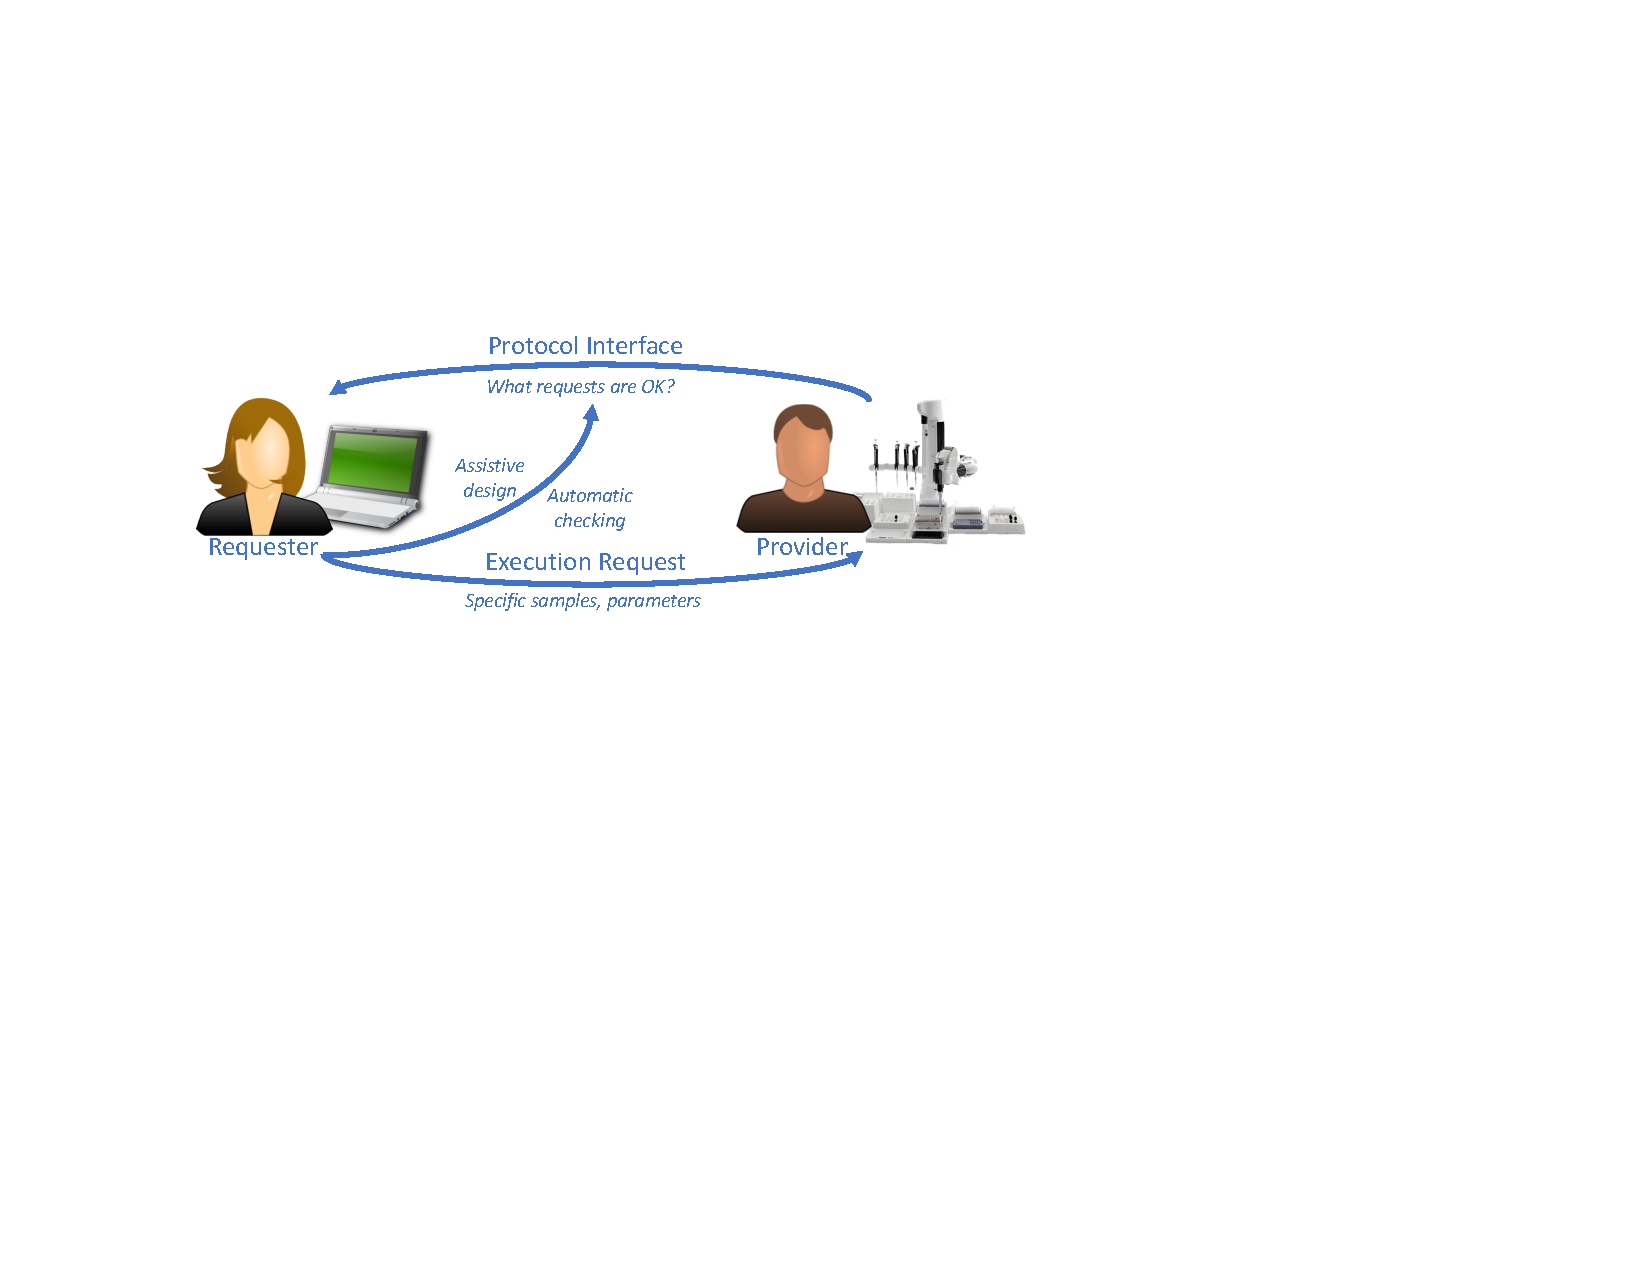
\includegraphics[width=0.8\textwidth]{figures/architecture.pdf}
\caption{OPIL connects experiment providers and requesters.}
\label{f:sequence}
\end{figure}

The Open Protocol Interface Language (OPIL) aims to address this problem by providing a data model to connect experiment providers and requesters.
Using OPIL, an experiment provider can provide a precise description of the protocols they offer, in terms of the options and constraints on the types of requests that can be made.
A requester can then use these interface descriptions to request the execution of a protocol on a specific set of samples with particular parameters.
OPIL can be applied both to automated protocols (e.g., via laboratory robotics or microfluidics) as well as to traditional human-executed ``paper'' protocols.

Where possible, OPIL builds on other existing standards.
In particular, OPIL uses the Synthetic Biology Open Language (SBOL) version 3~\citep{SBOL3} to describe biological samples in terms of combinations of strains, media, etc., and uses the Ontology of Units of Measure (OM) (\url{http://www.ontology-of-units-of-measure.org/resource/om-2}) to describe parameters with physical units.
Like these other standards, OPIL uses existing Semantic Web practices and resources, such as \emph{Uniform Resource Identifiers} (\opil{URI}s) and ontologies, to unambiguously identify and define biological system elements,
and to provide serialization formats for encoding this information in electronic data files.
This approach also allows OPIL to be extended with additional custom information for particular uses and deployments.

Note, however, that OPIL intentionally does not provide details about how the protocol works or guarantees about transfer or replicability of protocol executions. 
Likewise, OPIL is agnostic to any details of computer networking used to discover protocols or actually send requests.
OPIL focuses only on representing the minimal information for an unambiguous communication about requests to execute an offered protocol.



% % -----------------------------------------------------------------------------
\section{Overview of OPIL}
% % -----------------------------------------------------------------------------

In OPIL, a protocol is an activity that is configured with certain parameters and applied to a set of biological samples in order to produce a set of measurements by particular instruments at particular times, as illustrated in \ref{f:overview}.
An \opil{ExperimentalRequest} specifies a particular set of \opil{ParameterValue}s, \opil{SampleSet}s, and \opil{Measurement}s to be carried out. 
A \opil{ProtocolInterface} specifies which \opil{ExperimentalRequest}s are allowed for a given protocol with a parallel construction of \opil{Parameter}s, \opil{SampleSet}s, and \opil{MeasurementType}s

\begin{figure}[ht]
\begin{center}
  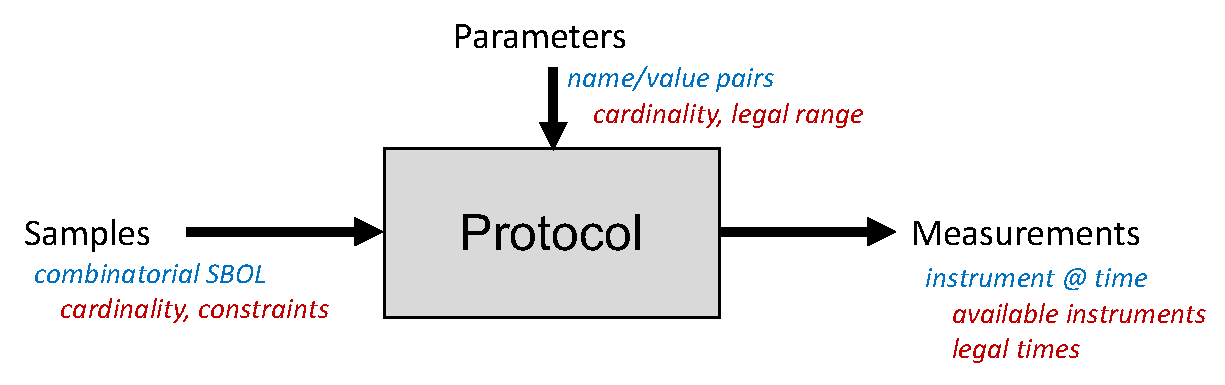
\includegraphics[scale=0.75]{figures/overview.pdf}
\caption{OPIL describes a request (blue) to execute a protocol in terms of samples, parameters, and measurements. 
A protocol interface (red) specifies what sorts of execution requests are allowed for that protocol.}
\label{f:overview}
\end{center}
\end{figure}

For example, consider a lab that is offering a multi-day bacterial protocol that might be described in prose as follows:
\begin{quote}
``Run either B. subtilis or E. coli samples in any media with up to 2 inducers for 1 to 4 days, sampling with a flow cytometer no more than once every 12 hours, and have the option of taking one RNAseq measurement. Culturing temperature is normally 37 C but can be set anywhere between 20 and 40 C.''
\end{quote}
These constraints could be encoded into a \opil{ProtocolInterface} by dividing them up as follows:
\begin{itemize}
\item Using \opil{SampleSet} objects: any {\it B. subtilis} or {\it E. coli} strain in any media, with up to 2 inducers.
\item Using \opil{Parameter} objects: run for 1-4 days, culture between 20-40 C with a default of 37 C.
\item Using \opil{MeasurementType} objects: any number of flow cytometer samples at least 12 hours apart, zero or one RNAseq measurement at any time.
\end{itemize}

An experimentalist who wishes to use this protocol might want to make a request such as the following:
\begin{quote}
``Please run all combinations of strains X and Y in media A, B, and C with 0, 0.1, 0.2, 0.5, and 1.0 uM arabinose. Run for 3 days with flow cytometry at hours 12, 30, 48, and 70. Culture at 27 C.''
\end{quote}
These specifies could be encoded into an \opil{ExperimentalRequest} by dividing them up as follows:
\begin{itemize}
\item Using \opil{SampleSet} objects: all combinations of strains X and Y in media A, B, and C with 0, 0.1, 0.2, 0.5, and 1.0 uM arabinose.
\item Using \opil{ParameterValue} objects: run for 3 days, culture at 27 C.
\item Using \opil{Measurement} objects: flow cytometry at hours 12, 30, 48, and 70.
\end{itemize}

The next sections provide complete definitions and details for all of these classes, along with more examples of their use.


% -----------------------------------------------------------------------------
\section{Conventions}
% -----------------------------------------------------------------------------

This section provides some preliminary information to aid in the understanding of the specification.
The SBOL data model is specified using Unified Modeling Language (UML) 2.0 diagrams \href{http://www.omg.org/spec/UML/2.0/}{(OMG 2005)}. This section reviews terminology conventions, the basics of UML diagrams, and our naming conventions.

\subsection{Terminology Conventions}

This document indicates requirement levels using the controlled vocabulary specified in \href{https://tools.ietf.org/html/rfc2119}{IETF RFC 2119}.
In particular, the key words ``MUST'', ``MUST NOT'', ``REQUIRED'', ``SHALL'', ``SHALL NOT'', ``SHOULD'', ``SHOULD NOT'', ``RECOMMENDED'', ``MAY'', and ``OPTIONAL'' in this document are to be interpreted as described in RFC 2119.

\begin{itemize}
\item The words ``MUST'', ``REQUIRED'', or ``SHALL'' mean that the item is an absolute requirement.
\item The phrases ``MUST NOT'' or ``SHALL NOT'' mean that the item is an absolute prohibition.
\item The word ``SHOULD'' or the adjective ``RECOMMENDED'' mean that there might exist valid reasons in particular circumstances to ignore a particular item, but the full implications need to be understood and carefully weighed before choosing a different course.
\item The phrases ``SHOULD NOT'' or ``NOT RECOMMENDED'' mean that there might exist valid reasons in particular circumstances when the particular behavior is acceptable or even useful, but the full implications needs to be understood and the case carefully weighed before implementing any behavior described with this label.
\item The word ``MAY'' or the adjective ``OPTIONAL'' mean that an item is truly optional.
\end{itemize}

\subsection{UML Diagram Conventions}
\label{sec:umldiagrams}

The types of data modeled by OPIL are commonly referred to as {\em classes}, especially when discussing the details of software implementation. Each OPIL class can be instantiated by many OPIL objects. These objects MAY contain data that differ in content, but they MUST agree on the type and form of their data as dictated by their common class. Classes are represented in UML diagrams as rectangles labeled at the top with class names (see \ref{fig:uml_sampler} for examples).

\begin{figure}[ht]
\begin{center}
  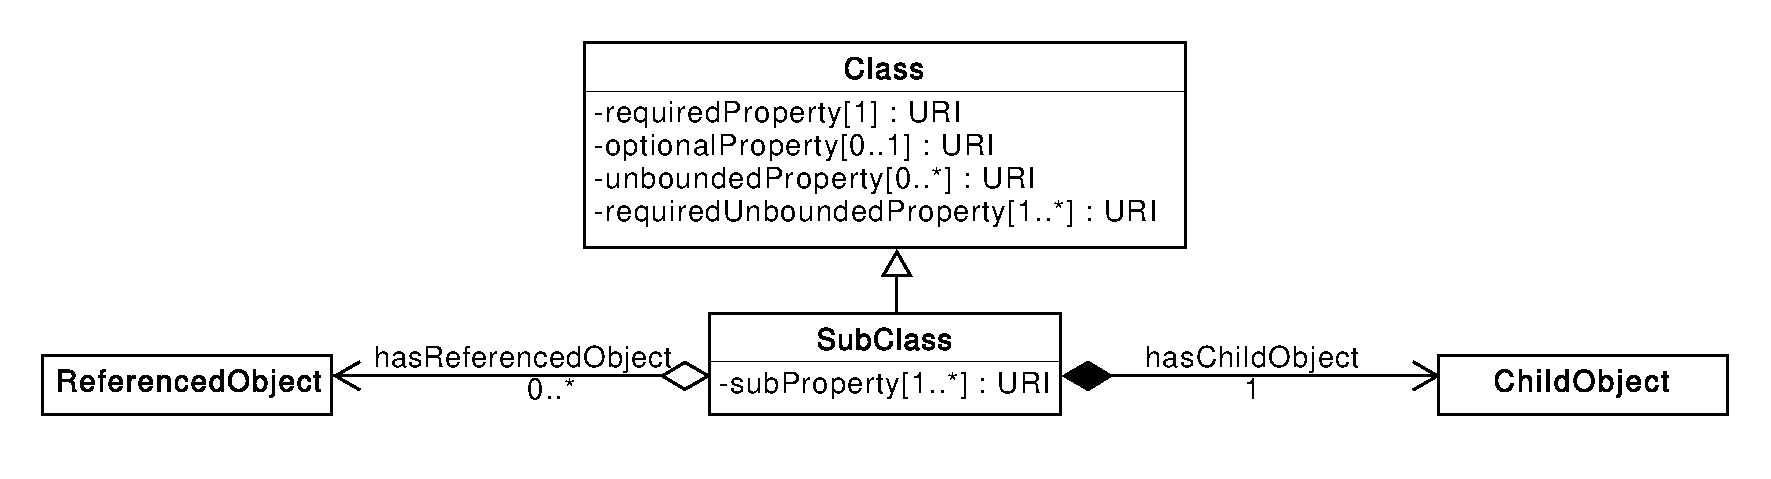
\includegraphics[width=\textwidth]{figures/uml_sampler.pdf}
\caption{Examples of UML diagram conventions used in this document}
\label{fig:uml_sampler}
\end{center}
\end{figure}

Classes can be connected to other classes by association properties, which are represented in UML diagrams as arrows. These arrows are labeled with data cardinalities in order to indicate how many values a given association property can possess (see below). The remaining (non-association) properties of a class are listed below its name. Each of the latter properties is labeled with its data type and cardinality.

In the case of an association property, the class from which the arrow originates is the owner of the association property. A diamond at the origin of the arrow indicates the type of association.
Open-faced diamonds indicate shared aggregation, also known as a reference, in which the owner of the association property exists independently of its value.

By contrast, filled diamonds indicate composite aggregation, also known as a part-whole relationship, in which the value of the association property MUST NOT exist independently of its owner.
In addition, in the OPIL data model, it is REQUIRED that the value of each composite aggregation property is a unique OPIL object (that is, not the value for more than one such property).
Note that in all cases, composite aggregation is used in such a way that there SHOULD NOT be duplication of such objects.
Such objects are also commonly referred to as ``child'' objects, and their owning objects as ``parent'' objects.

All OPIL properties are labeled with one of several restrictions on data cardinality. These are:

\begin{itemize}

\item $1$ - REQUIRED: there MUST be exactly one value for this property.

\item $0 \ldots 1$ - OPTIONAL: there MAY be a single value for this property, or it MAY be absent.

\item $0 \ldots *$ - zero or more: there MAY be any number of values for this property, including none.

\item $1 \ldots *$ - REQUIRED, one or more: there MAY be any number of values for this property, as long as there is at least one.

\item $n \ldots *$ - at least: there MUST be at least $n$ values for this property.

\end{itemize}

Finally, classes can inherit the properties of other classes. Inheritance relationships are represented in UML diagrams as open-faced, triangular arrows that point from the inheriting class to the inherited class. Some classes in the OPIL data model cannot be instantiated as objects and exist only to group common properties for inheritance. These classes have italicized names and are known as abstract classes.

\subsection{Naming and Typographic Conventions}
\label{sec:nameconventions}

OPIL classes are named using upper ``camel case,'' meaning that each word is capitalized and all words are run together without spaces, e.g., \opil{ProtocolInterface}.
Properties, on the other hand, are named using lower camel case, meaning that they begin lowercase but if they consist of multiple words, all words after the first begin with an uppercase letter (e.g., \opil{hasParameter}).

OPIL properties are always given singular names irrespective of their cardinality, e.g., \opil{hasParameter} is used rather than \opil{hasParameters} even though a \opil{ProtocolInterface} can have multiple parameters.
This is because each relation can potentially stand on its own, irrespective of the existence of others in the set.

Two conventions are used for property names, {\tt name} and {\tt hasName}.  
When a property is pointing to a class using the same name, it uses the {\tt hasName} convention (e.g., the \opil{ProtocolInterface} class uses \opil{hasParameter} to point to a \opil{Parameter} object).
When the property uses a different name than the class of the object it points to, it uses the {\tt name} convention instead (e.g., the \opil{MeasurementType} class uses \opil{minInterval} to point to a \opil{Measure} object).





% -----------------------------------------------------------------------------
\section{SBOL Imports: Identifiers, Primitive Types, and Classes}
% -----------------------------------------------------------------------------

OPIL builds on the Synthetic Biology Open Language (SBOL) version 3~\citep{SBOL3} in several ways:
\begin{itemize}
\item OPIL uses the same conventions as SBOL for URIs and types.
\item OPIL uses the SBOL base classes \sbol{Identified} and \sbol{TopLevel} as parents for all OPIL classes.
\item OPIL uses SBOL classes to describe biological samples in terms of combinations of strains, media, etc.
\item OPIL makes use of the same external measurement ontology as SBOL, the Ontology of Units of Measure (OM) (\url{http://www.ontology-of-units-of-measure.org/resource/om-2}).
\end{itemize}

In order to make this document more self-contained, this section repeats the material from the SBOL specification on conventions and SBOL base classes.
A summary is also provided for key SBOL and OM classes; for complete documentation, see the SBOL specification.
In case of conflict between any material in this section and the SBOL specification, the SBOL specification should be held correct.

\subsection{Uniform Resource Identifiers}
\label{sec:URIstructure}

As OPIL is built upon the Resource Description Framework (RDF), all class instances are identified by a Uniform Resource Identifier (URI).  In the OPIL data model, the value of an association property MUST be a \opil{URI} or set of \opil{URI}s that refer to OPIL objects belonging to the class at the tip of the arrow.  Every \sbol{Identified} object's URI MUST be globally unique among all other \sbol{Identified} object URIs. It is also highly RECOMMENDED that the \opil{URI} structure follows the recommended best practices for compliant \opil{URI}s specified in \ref{sec:compliant}.

Whenever a \sbol{TopLevel} object's URI is a URL (e.g., following the conventions of HTTP(S) rather than a UUID), its structure MUST comply with the following rules:

\begin{itemize}

 \item A \sbol{TopLevel} URL MUST use the following pattern:
  \texttt{[namespace]/[local]/[displayId]},  where \texttt{namespace} and \sbol{displayId} are required fragments, and the \texttt{local} fragment is an optional relative path.
  
  	For example, a \opil{ProtocolInterface} might have the URL~\path{https://igem.org/protocols/OD/calibration_2018}, where \texttt{namespace} is \path{https://igem.org}, \texttt{local} is \path{protocols/OD}, and \sbol{displayId} is \path{calibration_2018}.

  \item A \sbol{TopLevel} object's URL MUST NOT be included as prefix for any other \sbol{TopLevel} object.
  
  	For example, the \path{run102} \opil{ExecutionRequest} object cannot have a URL of \path{https://igem.org/protocols/OD/calibration_2018/run102}, since the \path{https://igem.org/protocols/OD/calibration_2018} prefix is already used as a URL for the \path{calibration_2018} \opil{ProtocolInterface} object.

  \item The URL of any child or nested object MUST use the following pattern:\texttt{[parent]/[displayId]}, where \texttt{parent} is the URL of its parent object.
	Multiple layers of child objects are allowed using the same\\ \texttt{[parent]/[displayId]} pattern recursively.
	
	For example, a \opil{MeasurementType} object owned by the \path{calibration_2018} \opil{ProtocolInterface} and having a \sbol{displayId} of \texttt{MeasurementType1} will have a URL of \path{https://igem.org/protocols/OD/calibration_2018/MeasurementType1}.
	Similarly, if the \texttt{MeasurementType1} object has a \opil{TimeInterval} child object with a \sbol{displayId} of \texttt{TimeInterval1}, then that object will have the URL\\ \path{https://igem.org/protocols/OD/calibration_2018/MeasurementType1/TimeInterval1}.
  \end{itemize}

\subsubsection{Compliant URIs}
\label{sec:compliant}

Maintaining unique URIs for objects can be challenging.  Compliant URIs follow a set of rules that simplify this challenge.

Compliant URIs for \sbol{TopLevel} objects MUST conform to the following pattern:
\begin{quotation} 
\refObj{namespace}/\refObj{collection\_structure}/\refObj{displayId}
\end{quotation}

The \refObj{namespace} token MAY further decompose into \refObj{domain}/\refObj{root} tokens. The \refObj{root} and \refObj{collection\_structure} tokens may optionally be omitted; alternatively, they may consist of an arbitrary number of delimiter-separated layers. Note that this pattern means that SBOL-compliant \opil{URI}s can be automatically decomposed with the aid of a \sbol{TopLevel} object's \sbol{hasNamespace} property. SBOL-compliant objects can be easily remapped into new namespaces by changing only the \refObj{namespace}.

Consider, for example, the SBOL-compliant \opil{URI}:
\begin{quote}``https://igem.org/engineering/protocols/platereader/OD/calibration\_2018''\end{quote} 
for a \sbol{Component} with a \sbol{hasNamespace} value ``https://igrem.org/engineering/protocols''.
This \opil{URI} can be decomposed as follows:
\begin{quote} 
namespace: ``https://igrem.org/engineering/protocols'' \linebreak
domain: ``https://igem.org'' \linebreak
root: ``engineering/protocols'' \linebreak
collection: ``platereader/OD'' \linebreak
displayId: ``calibration\_2018'' \linebreak
\end{quote}

SBOL-compliant URIs also facilitate auto-construction of child objects with unique \opil{URI}s. 
Child objects of \sbol{TopLevel} objects with compliant \opil{URI}s MUST conform to the following pattern:\\ ``\refObj{parent\_uri}/\refObj{child\_type}\refObj{child\_type\_counter}'' where the \refObj{parent\_uri} refers to the URI of the parent object, the \refObj{child\_type} refers to the SBOL class of the child object, and \refObj{child\_type\_counter} is a unique index for the child object. 
The \refObj{child\_type\_counter} of a new object SHOULD be calculated at time of object creation as 1 + the maximum \refObj{child\_type\_counter} for each \refObj{child\_type} object in the parent (e.g., ``\refObj{parent\_uri}/Parameter7''). 
Note that numbering is independent for each type, so a \opil{ProtocolInterface} can have children ``Parameter7'' and ``MeasurementType7''.

\subsection{OPIL URIs}
 \label{sec:sbolURIs}
  
\todo[inline]{This needs to be changed from BBN to a more general community name and given a version number}
The SBOL namespace, which is \url{http://bbn.com/synbio/opil\#}, is used to indicate which entities and properties in an OPIL document are defined by OPIL. 
For example, the URI of the type \opil{ProtocolInterface} is \url{http://bbn.com/synbio/opil\#ProtocolInterface}. 
This convention is assumed throughout the specification.
The OPIL namespace MUST NOT be used for any entities or properties not defined in this specification.  

Other namespaces are also used by OPIL, however, notably the SBOL 3 namespace \url{http://sbols.org/v3\#}, as well as other namespaces used by SBOL including Dublin Core~\citep{dcmi2012}), Ontology of Units of Measure (OM), and various biological ontologies.


\subsection{Primitive Data Types}
\label{sec:datatypes}
\label{sec:string}
\label{sec:integer}
\label{sec:long}
\label{sec:float}
\label{sec:boolean}
\label{sec:URI}
\label{sec:literal}

When OPIL uses simple ``primitive'' data types such as \opil{string}s or \opil{integer}s, these are defined as the following specific formal types:
\begin{itemize}
\item \opil{string}: \url{http://www.w3.org/2001/XMLSchema\#string}\\
  {\em Example: ``LacI coding sequence''}
\item \opil{integer}: \url{http://www.w3.org/2001/XMLSchema\#integer}\\
  {\em Example: 3}
\item \opil{long}: \url{http://www.w3.org/2001/XMLSchema\#long}\\
  {\em Example: 9223372036854775806}
\item \opil{float}: \url{http://www.w3.org/2001/XMLSchema\#float}\\
  {\em Example: 3.14159}
\item \opil{boolean}: \url{http://www.w3.org/2001/XMLSchema\#boolean}\\
  {\em Example: \external{true}}
\end{itemize}

The term \opil{literal} is used to denote an object that can be any of the five types listed above.

In addition to the simple types listed above, OPIL also uses objects with types \emph{Uniform Resource Identifier} (\opil{URI}). It is important to realize that in RDF, a \opil{URI} might or might not be a resolvable URL (web address).  A \opil{URI} is always a globally unique identifier within a structured namespace.  In some cases, that name is also a reference to (or within) a document, and in some cases that document can also be retrieved (e.g., using a web browser).

\subsection{OPIL Types}
\label{sec:sbolTypes}

\todo[inline]{Change to match above when root namespace changes: perhaps bioprotocols.org?}
All OPIL objects are given the most specific \external{rdfType} in the OPIL namespace (\uri{http://bbn.com/synbio/opil\#}) that defines the type of the object.  Namely, an object MUST have no more than one \external{rdfType} property in the \uri{http://bbn.com/synbio/opil\#} namespace.

For example, an object cannot have both the \external{rdfType} of \opil{ProtocolInterface} and \opil{MeasurementType}.  Also, a \opil{MeasureParameter} would have this \external{rdfType} and not also include \external{rdfType}s for classes that it inherits from, such as \opil{Parameter} and \sbol{Identified}.

\subsection{SBOL Classes}

OPIL classes use \sbol{Identified} and \sbol{TopLevel} as their root classes.
The OPIL \opil{SampleSet} class extends the \sbol{CombinatorialDerivation} class and makes use of the \sbol{Component} class to describe the composition of experimental samples.
This subsection summarizes the minimum information required to use these SBOL classes in OPIL; for full details, see the Synthetic Biology Open Language (SBOL) version 3 specification~\citep{SBOL3}

\subsubsection{sbol:Identified}
\label{sec:sbol:Identified}

All OPIL- and SBOL-defined classes are directly or indirectly derived from the \sbol{Identified}  abstract class.
This inheritance means that all OPIL and SBOL objects are uniquely identified using \opil{URI}s that uniquely refer to these objects within an SBOL document or at locations on the World Wide Web.

As shown in \ref{uml:identified}, the \sbol{Identified} class includes the following properties: \sbol{displayId},  \sbol{name}, \sbol{description}, \prov{wasDerivedFrom}, and \prov{wasGeneratedBy}. 

\begin{figure}[ht]
\begin{center}
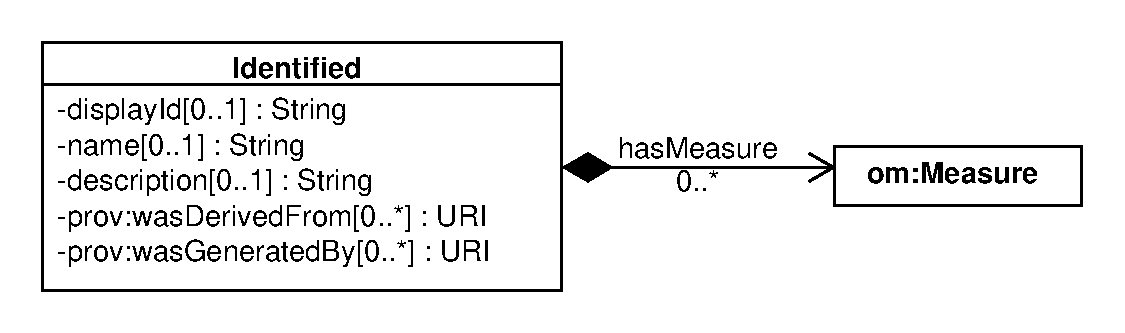
\includegraphics[scale=0.6]{sbol_uml/identified}
\caption[]{Diagram of the \sbol{Identified} abstract class and its associated properties}
\label{uml:identified}
\end{center}
\end{figure}

\begin{itemize}
\item \label{sec:sbol:displayId} 
The \sbol{displayId} property is an OPTIONAL identifier with a data type of \opil{string} (and REQUIRED for objects with URL identifiers). This property is intended to be an intermediate between a URI and the \sbol{name} property that is machine-readable, but more human-readable than the full URI of an object.
If set, its \opil{string} value MUST be composed of only alphanumeric or underscore characters and MUST NOT begin with a digit.

\item \label{sec:sbol:name}
The \sbol{name} property is OPTIONAL and has a data type of \opil{string}. This property is intended to be displayed to a human when visualizing an \sbol{Identified} object.
If an \sbol{Identified} object lacks a name, then software tools SHOULD instead display the object's \sbol{displayId} or URI.

\item \label{sec:sbol:description}
The \sbol{description} property is OPTIONAL and has a data type of \opil{string}. This property is intended to contain a more thorough text description of an \sbol{Identified} object.

\item \label{sec:prov:wasDerivedFrom}
The \prov{wasDerivedFrom} property MAY contain any number of \opil{URI}s. This property is defined by the PROV-O ontology and is located in the \url{https://www.w3.org/ns/prov#} namespace.

\item \label{sec:prov:wasGeneratedBy}
The \prov{wasGeneratedBy} property MAY contain any number of \opil{URI}s. This property is defined by the PROV-O ontology and is located in the \url{https://www.w3.org/ns/prov#} namespace.

\item \label{sec:sbol:hasMeasure}
The \sbol{hasMeasure} property MAY contain any number of \opil{URI}s, each of which refers to a \om{Measure} object that describes a measured parameter for this object.
\end{itemize}

\subsubsection{sbol:TopLevel}
\label{sec:sbol:TopLevel}

\sbol{TopLevel} is an abstract class that is extended by any \sbol{Identified} class that can be found at the top level of an OPIL or SBOL document or file.
In other words, \sbol{TopLevel} objects are never nested inside of any other object as a child object.
The \sbol{TopLevel} classes defined in OPIL are \opil{ProtocolInterface} and \opil{ExperimentRequest}. 

\begin{figure}[ht]
\begin{center}
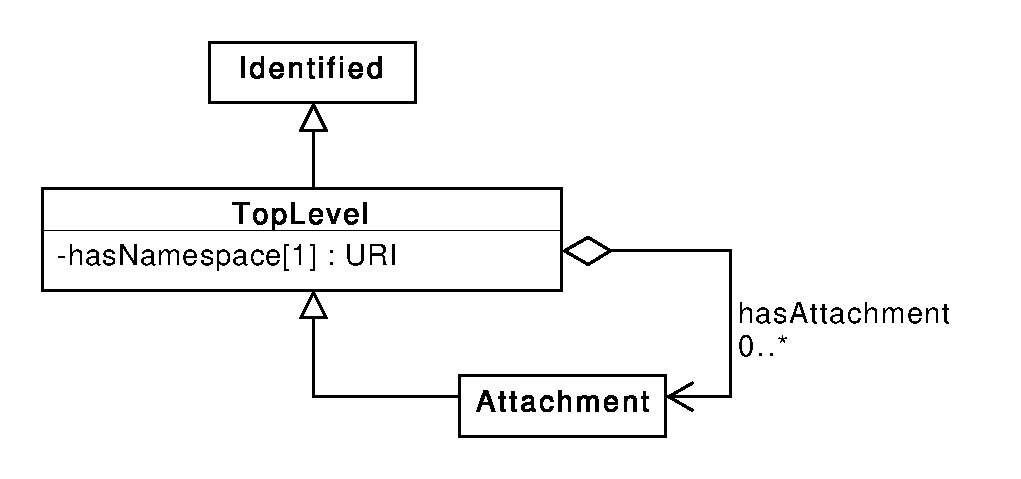
\includegraphics[scale=0.6]{sbol_uml/toplevel}
\caption[]{Classes that inherit from the \sbol{TopLevel} abstract class.}
\label{uml:toplevel}
\end{center}
\end{figure}

\begin{itemize}
\item \label{sec:sbol:hasNamespace}
The \sbol{hasNamespace} property is REQUIRED and MUST contain a single \opil{URI} that defines the namespace portion of URLs for this object and any child objects.
If the URI for the \sbol{TopLevel} object is a URL, then the URI of the \sbol{hasNamespace} property MUST prefix match that URL.

\item 
\label{sec:sbol:hasAttachment}
The \sbol{hasAttachment} property MAY have any number of \opil{URI}s, each referring to an \sbol{Attachment} object.
\end{itemize}


\subsubsection{sbol:Component}
\label{sec:sbol:Component}

The \sbol{Component} class represents the structural and/or functional entities of a biological design. 
In OPIL, this is primarily used to represent the design of experimental samples as combinations of entities such as strains, genetic constructs, media, inducers, etc.

As shown in \ref{uml:component}, the \sbol{Component} class describes a design entity using a number of different properties.
In many OPIL usages, however, the only properties required will be \sbolmult{type:C}{type} and \sbol{hasFeature}.

\begin{figure}[ht]
\begin{center}
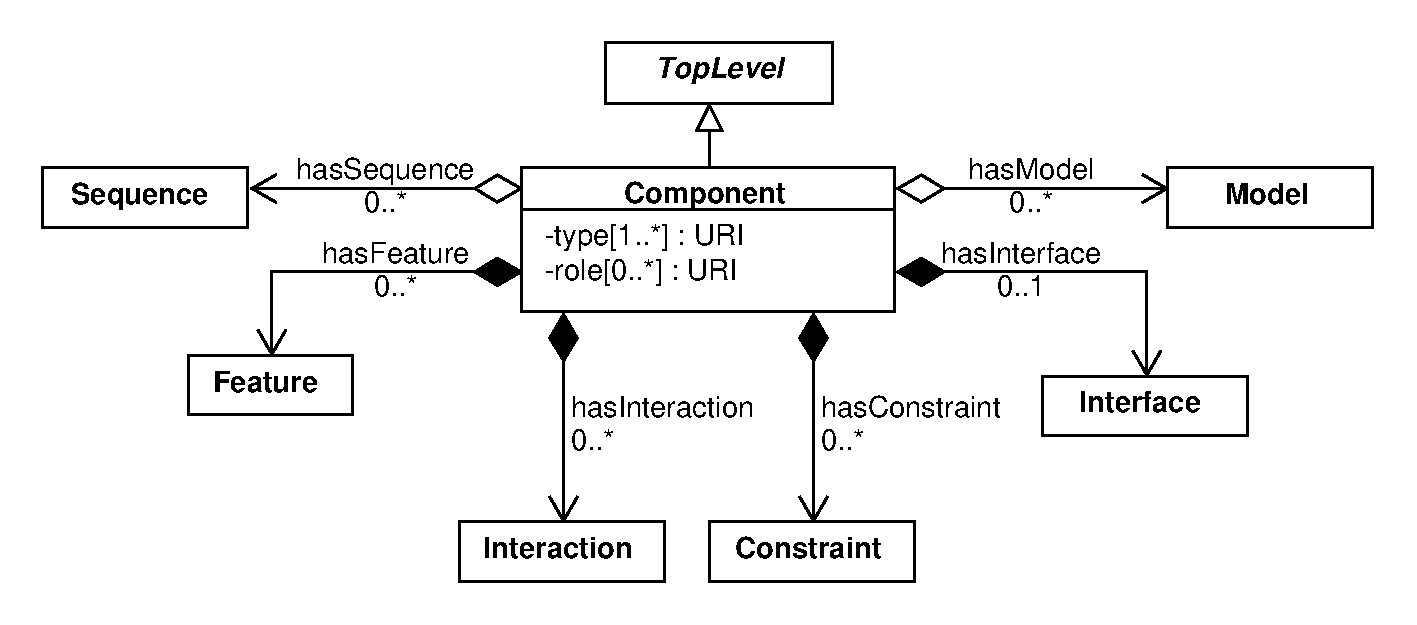
\includegraphics[scale=0.6]{sbol_uml/component}
\caption[]{Diagram of the \sbol{Component} class and its associated properties.}
\label{uml:component}
\end{center}
\end{figure} 

\begin{itemize}
\item \label{sec:sbol:type:C}
The \sbolmult{type:C}{type} property MUST have one or more \opil{URI}s specifying the category of biochemical or physical entity (for example DNA, protein, or simple chemical) that a \sbol{Component} object represents.
For OPIL, this SHOULD be from the physical entity representation branch of the Systems Biology Ontology~\citep{SBO}
and will typically be Functional Entity (\url{https://identifiers.org/SBO:0000241}), which is used to systems of multiple interacting molecules.

\item \label{sec:sbol:hasFeature}
The \sbol{hasFeature} property MAY have any number of \opil{URI}s, each referencing a \sbol{Feature} object. Each \sbol{Feature} represents a specific occurrence of a part, subsystem, or other notable aspect within that design, such as an ingredient in the composition of a growth medium.

\item \label{sec:sbol:role:C}
The \sbolmult{role:C}{role} property MAY have any number of \opil{URI}s, which MUST identify terms from ontologies that are consistent with the \sbolmult{type:C}{type} property of the \sbol{Component}. 
\\{\em This is not typically required for specifying experimental sample designs in OPIL.}

\item \label{sec:sbol:hasSequence:C}
The \sbolmult{hasSequence:C}{hasSequence} property MAY have any number of \opil{URI}s, each referencing a \sbol{Sequence} object.  These objects define the primary structure or structures of the \sbol{Component}.
\\{\em This is not typically required for specifying experimental sample designs in OPIL.}

\item \label{sec:sbol:hasConstraint}
The \sbol{hasConstraint} property MAY have any number of \opil{URI}s, each referencing a \sbol{Constraint} object.
These objects describe, among other things, any restrictions on the relative, sequence-based positions and/or orientations of the \sbol{Feature} objects contained by the \sbol{Component}, as well as spatial relations such as containment and identity relations.
\\{\em This is not typically required for specifying experimental sample designs in OPIL.}

\item \label{sec:sbol:hasInteraction}
The \sbol{hasInteraction} property MAY have any number of \opil{URI}s, each referencing an \sbol{Interaction} object describing a behavioral relationship between \sbol{Feature}s in the \sbol{Component}.
\\{\em This is not typically required for specifying experimental sample designs in OPIL.}

\item \label{sec:sbol:hasInterface}
The \sbol{hasInterface} property is OPTIONAL and MAY have a \opil{URI} referencing an \sbol{Interface} object that indicates the inputs, outputs, and non-directional points of connection to a \sbol{Component}.
\\{\em This is not typically required for specifying experimental sample designs in OPIL.}

\item \label{sec:sbol:hasModel}
The \sbol{hasModel} property MAY have any number of \opil{URI}s, each referencing a \sbol{Model} object that links the \sbol{Component} to a computational model in any format.
\\{\em This is not typically required for specifying experimental sample designs in OPIL.}
\end{itemize}

\subsubsection{Feature}
\label{sec:sbol:Feature}

The \sbol{Feature} class, as shown in \ref{uml:subcomponent} is used to define the structure of \sbol{Component} objects.
In OPIL, the \sbol{Feature} subclasses most often used will be \sbol{LocalSubComponent} and \sbol{ExternallyDefined}

\begin{figure}[ht]
\begin{center}
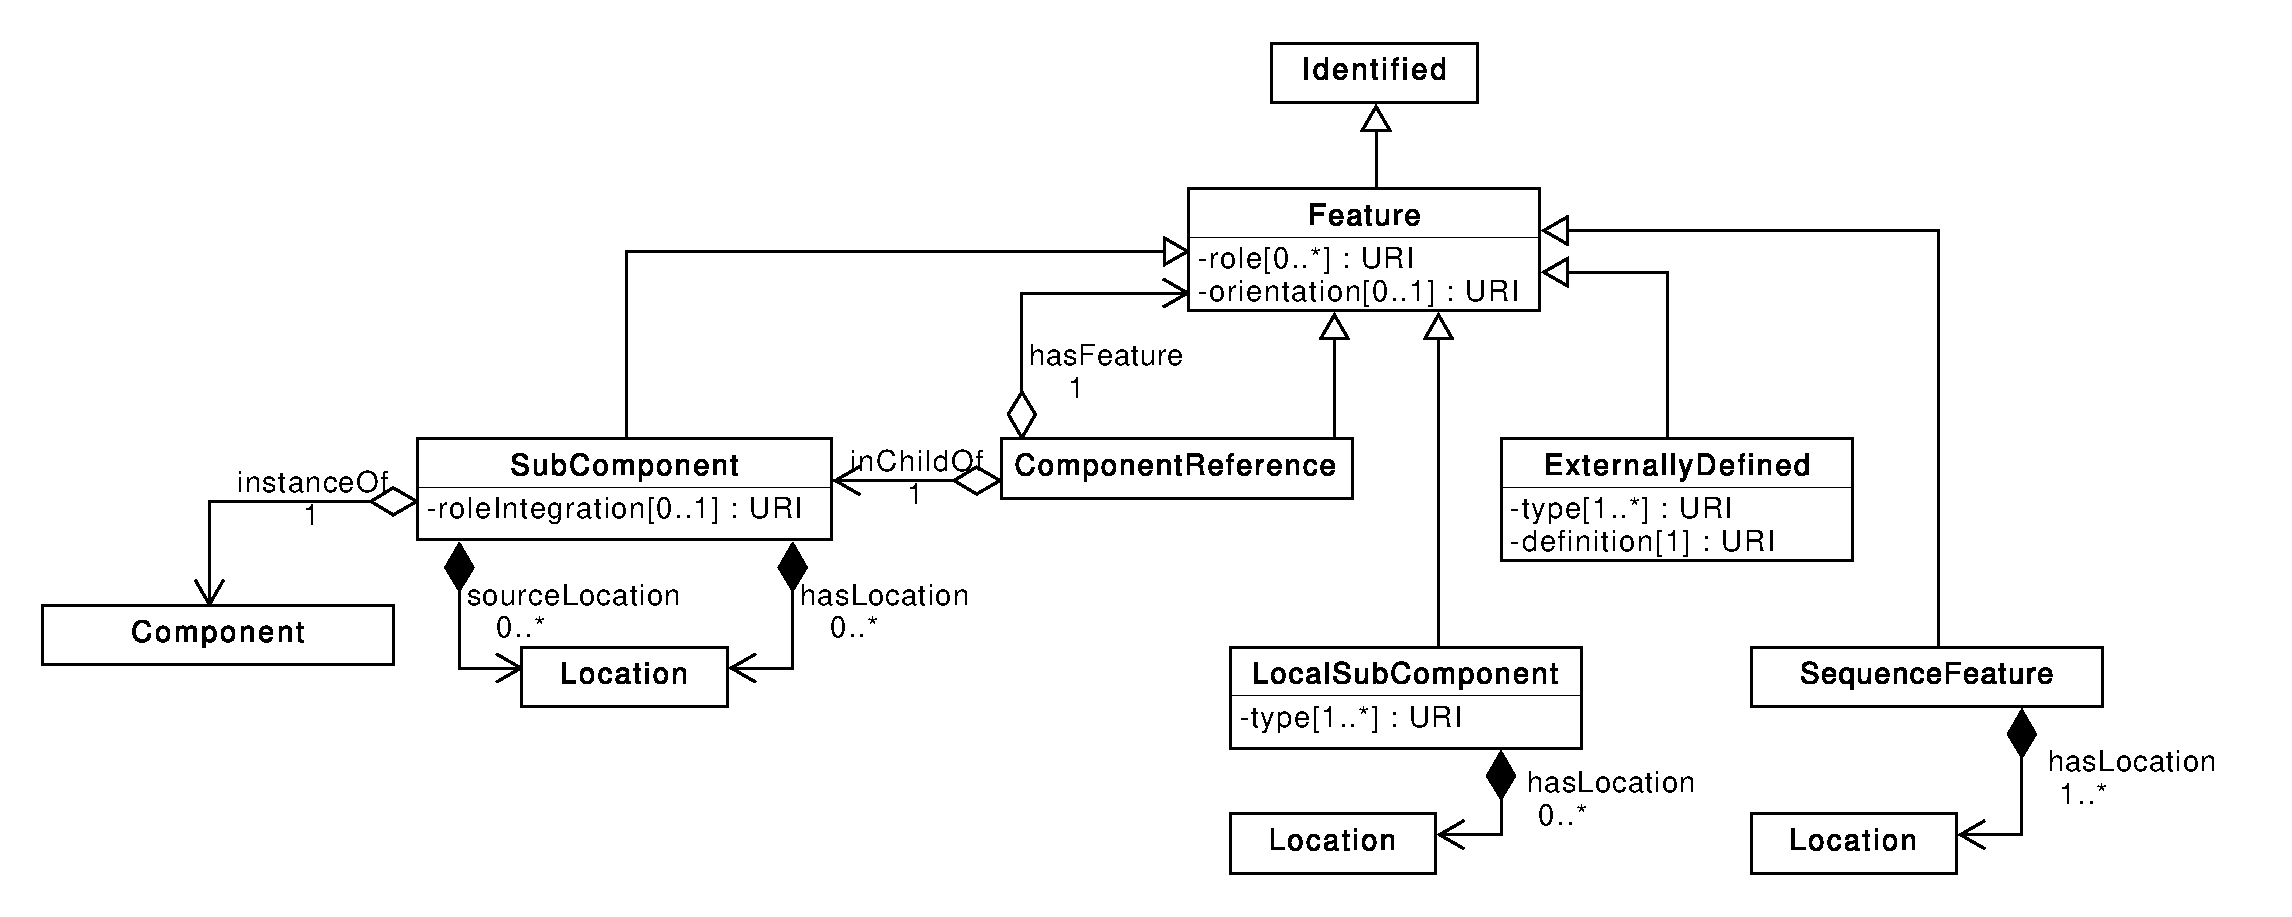
\includegraphics[width=\textwidth]{sbol_uml/feature}
\caption[]{Diagram of the \sbol{Feature} class, its children, and associated properties.}
\label{uml:subcomponent}
\end{center}
\end{figure}

\begin{itemize}
\item \label{sec:sbol:role:F}
The \sbolmult{role:F}{role} property MAY have any number of \opil{URI}s describing the purpose or potential function of this \sbol{Feature} in the context of its parent \sbol{Component}.
\\{\em This is not typically required for specifying experimental sample designs in OPIL.}

\item \label{sec:sbol:orientation:F}
The \sbolmult{orientation:F}{orientation} property is OPTIONAL and has a data type of \opil{URI}. It is used to indicate the orientation of a double-stranded \sbol{Feature} with respect to a \sbol{Sequence} in its parent \sbol{Component}.
\\{\em This is not typically required for specifying experimental sample designs in OPIL.}
\end{itemize}

\paragraph{LocalSubComponent}
\label{sec:sbol:LocalSubComponent}

The \sbol{LocalSubComponent} class is a subclass of \sbol{Feature}. 
This class serves as a way to create a placeholder in more complex \sbol{Component}s, such as a variable to be filled in later or a composite that exists only within the context of the parent \sbol{Component}.

In OPIL, this is typically used to specify a variable in a sample design, such as a strain to be varied, or to specify fixed components best described in SBOL, such as a genetic construct.

\begin{itemize}
\item \label{sec:sbol:type:LSC}
The \sbolmult{type:LSC}{type} property is REQUIRED and contains one or more \opil{URI}s. The \sbolmult{type:LSC}{type} property is identical to its use in \sbol{Component}.

\item \label{sec:sbol:hasLocation:LSC}
The \sbolmult{hasLocation:LSC}{hasLocation} property MAY have any number of \opil{URI}s, each refering to a \sbol{Location} object that indicates the position of this \sbol{Feature} within a \sbol{Sequence} associated with the parent \sbol{Component}.
\\{\em This is not typically required for specifying experimental sample designs in OPIL.}
\end{itemize}

\paragraph{ExternallyDefined}
\label{sec:sbol:ExternallyDefined}

The \sbol{ExternallyDefined} class defined features by reference to external databases like ChEBI or UniProt.

In OPIL, this is typically used to specify fixed elements of a sample design that are well-described by a non-SBOL resource, such as inducers, carbon sources, and antibiotics.

\begin{itemize}
\item \label{sec:sbol:type:ED}
The \sbolmult{type:ED}{type} property is REQUIRED and contains one or more \opil{URI}s. The \sbolmult{type:ED}{type} property is identical to its use in \sbol{Component}.

\item \label{sec:sbol:definition:ED}
The \sbolmult{definition:ED}{definition} property is REQUIRED and contains a \opil{URI} that links to a canonical definition external to SBOL and OPIL.
When possible, such definitions SHOULD use the recommended external resources in \ref{sec:recomm_ontologies}.
For example, an \sbol{ExternallyDefined} simple chemical might link to ChEBI and a protein might link to UniProt.
\end{itemize}

\paragraph{SubComponent}
\label{sec:sbol:SubComponent}

The \sbol{SubComponent} class is a subclass of the \sbol{Feature} class that can be used to specify structural hierarchy.
For example, the \sbol{Component} of a gene might contain four \sbol{SubComponent} objects: a promoter, RBS, CDS, and terminator, each linked to a \sbol{Component} that provides the complete definition.
\\{\em This is not typically required for specifying experimental sample designs in OPIL.}

\paragraph{ComponentReference}
\label{sec:sbol:ComponentReference}

The \sbol{ComponentReference} class is a subclass of \sbol{Feature} that can be used to reference \sbol{Feature}s within \sbol{SubComponent}s. 
\\{\em This is not typically required for specifying experimental sample designs in OPIL.}

\paragraph{SequenceFeature}
\label{sec:sbol:SequenceFeature}

The \sbol{SequenceFeature} class describes one or more regions of interest on the \sbol{Sequence} objects referred to by its parent \sbol{Component}. 
\\{\em This is not typically required for specifying experimental sample designs in OPIL.}

\subsubsection{CombinatorialDerivation}
\label{sec:sbol:CombinatorialDerivation}

The purpose of the \sbol{CombinatorialDerivation} class is to specify combinatorial biological designs without having to specify every possible design variant. 
In OPIL, this is used to specify experiment designs that vary different factors.
For example, a \sbol{CombinatorialDerivation} can be used to specify an experiment that tests the growth of one of four different strains growing on five carbon sources at two different temperatures, thus specifying a total of 40 different combinations of experimental conditions.

\begin{figure}[ht]
\begin{center}
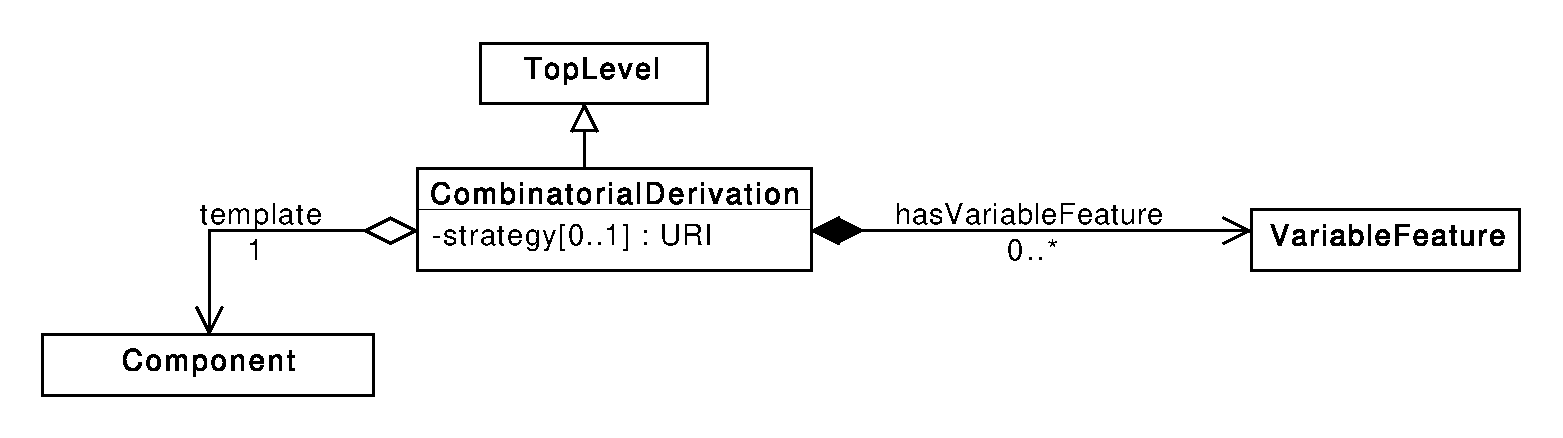
\includegraphics[scale=0.6]{sbol_uml/combinatorial_derivation}
\caption[]{Diagram of the \sbol{CombinatorialDerivation} class and its associated properties.}
\label{uml:combinatorial_derivation}
\end{center}
\end{figure}

\begin{itemize}
\item \label{sec:sbol:template}
The \sbol{template} property is REQUIRED and MUST contain a URI that refers to a \sbol{Component}. 
This \sbol{Component} is expected to serve as a template for the derivation of new \sbol{Component} objects. 
Consequently, its \sbol{hasFeature} properties SHOULD contain one or more \sbol{Feature} objects that describe its substructure (referred to hereafter as template \sbol{Feature} objects), and its other properties MAY also describe other aspects of the template that will not change based on the values that may be varied.

\item \label{sec:sbol:hasVariableFeature}
The \sbol{hasVariableFeature} property can have any number of \opil{URI}s, each referring to a \\ \sbol{VariableFeature} that defines the set of possible values for one of the variables in the \sbol{template}.
The set of \sbol{hasVariableFeature} properties MUST NOT contain two or more \sbol{VariableFeature} objects that refer to the same template \sbol{Feature} via their \sbol{variable} properties (i.e., do not define the same variable twice).

\item \label{sec:sbol:strategy}
The \sbol{strategy} property is OPTIONAL and has a data type of \opil{URI}. \ref{tbl:strategy} provides a list of REQUIRED \sbol{strategy} URIs. If the \sbol{strategy} property is not empty, then it MUST contain a URI from \ref{tbl:strategy}. This property recommends how many \sbol{Component} objects SHOULD be derived from the template \sbol{Component}.
\\{\em In OPIL, this will typically be \url{http://sbols.org/v3#enumerate} for most experiments.}
\end{itemize}

\begin{table}[ht]
  \begin{edtable}{tabular}{lp{4in}}
    \toprule
    \textbf{Strategy URI} & \textbf{Description} \\
    \midrule
    \url{http://sbols.org/v3#enumerate}  &  Derivation SHOULD produce all possible \sbol{Component} objects specified by the \sbol{CombinatorialDerivation}. \\
        \url{http://sbols.org/v3#sample}  & Derivation SHOULD produce a subset of possible \sbol{Component} objects specified by \sbol{CombinatorialDerivation}. The manner in which this subset is chosen is left unspecified. \\
    \bottomrule
  \end{edtable}
  \caption{REQUIRED \opil{URI}s for the \sbol{strategy} property.}
  \label{tbl:strategy}
\end{table}

\subsubsection{VariableFeature}
\label{sec:sbol:VariableFeature}

As described \sbolmult{hasVariableFeature}{above}, the \sbol{VariableFeature} class specifies a variable and a set of values for that variable.

When the values are set by the \sbol{variant}, \sbol{variantCollection}, and \sbol{variantDerivation} properties, they specify the different design elements that {\em replace} the \sbol{Feature} specified by the \sbol{variable} property.
For example, a set of \sbol{variant} values might indicate three media, one of which will be used for each sample.

When the values are set by the \sbol{variantMeasure} property, they specify the different quantities for the \sbol{Feature} specified by the \sbol{variable} property.
For example, a set of \sbol{variantMeasure} values might indicate five different concentrations to use for an inducer.

\begin{figure}[ht]
\begin{center}
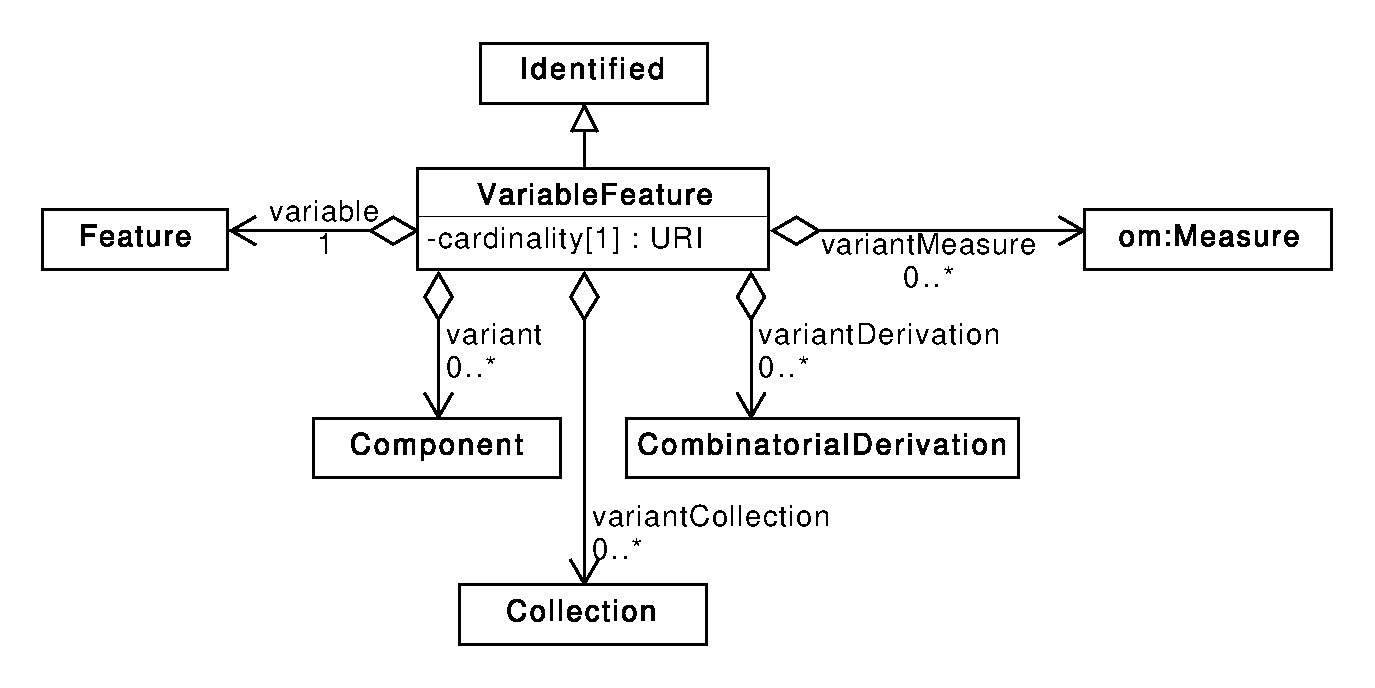
\includegraphics[scale=0.6]{sbol_uml/variable_component}
\caption[]{Diagram of the \sbol{VariableFeature} class and its associated properties.}
\label{uml:variable_component}
\end{center}
\end{figure}

\begin{itemize}
\item \label{sec:sbol:variable}
The \sbol{variable} property is REQUIRED and MUST contain a \opil{URI} that refers to a template \sbol{Feature} in the \sbol{template} \sbol{Component} referred to by this \sbol{VariableFeature}'s parent \\ \sbol{CombinatorialDerivation}.

\item \label{sec:sbol:variantMeasure}
The \sbol{variantMeasure} property MAY have any number of \opil{URI}s, each referring to a \om{Measure} object. This property specifies numerical values that are options for \sbol{hasMeasure} property values for the \sbol{variable} \sbol{Feature} from the \sbol{template}.

\item \label{sec:sbol:variant}
The \sbol{variant} property MAY have any number of \opil{URI}s, each referring to a \sbol{Component} object. This property specifies individual \sbol{Component} objects to serve as options for replacing the \sbol{variable} \sbol{Feature} from the \sbol{template}.

\item \label{sec:sbol:variantCollection}
The \sbol{variantCollection} property MAY have any number of \opil{URI}s, each referring to a \sbol{Collection} object.
Such a \sbol{Collection} MUST NOT contain any objects besides \sbol{Component} objects or \sbol{Collection} objects that themselves contain only \sbol{Component} or \sbol{Collection} objects.
This property enables the specification of groups of \sbol{Component} objects to serve as options.

\item \label{sec:sbol:variantDerivation}
The \sbol{variantDerivation} property MAY have any number of \opil{URI}s, each referring to a \\ \sbol{CombinatorialDerivation} object. 
This property enables the specification of \sbol{Component} objects derived in accordance with another \sbol{CombinatorialDerivation} to serve as options for the \sbol{variable} \sbol{Feature} from the \sbol{template}. 

\item \label{sec:sbol:cardinality}
The \sbol{cardinality} property is REQUIRED and has type of \opil{URI}. This property specifies how many \sbol{Feature} objects SHOULD be derived from the template \sbol{Feature} during the derivation of a new \sbol{Component}. The URI value of this property MUST come from the URIs provided in~\ref{tbl:cardinality}.
\\{\em In OPIL, this will typically be \url{http://sbols.org/v3#one} for most experiments.}

\begin{table}[ht]
  \begin{edtable}{tabular}{lp{4in}}
    \toprule
    \textbf{Cardinality URI} & \textbf{Description} \\
    \midrule
    \url{http://sbols.org/v3#zeroOrOne} & No more than one \sbol{Feature} in the derived \sbol{Component} SHOULD have a \prov{wasDerivedFrom} property that refers to the template \sbol{Feature}. \\
        \url{http://sbols.org/v3#one} & Exactly one \sbol{Feature} in the derived \sbol{Component} SHOULD have a \prov{wasDerivedFrom} property that refers to the template \sbol{Feature}. \\
\url{http://sbols.org/v3#zeroOrMore} & Any number of \sbol{Feature} objects in the derived \sbol{Component} MAY have \prov{wasDerivedFrom} properties that refer to the template \sbol{Feature}. \\
\url{http://sbols.org/v3#oneOrMore} & At least one \sbol{Feature} in the derived \sbol{Component} SHOULD have a \prov{wasDerivedFrom} property that refers to the template \sbol{Feature}. \\
    \bottomrule
  \end{edtable}
  \caption{REQUIRED \opil{URI}s for the \sbol{cardinality} property.}
  \label{tbl:cardinality}
\end{table}


\end{itemize}

\subsection{Ontology of Units of Measure}

In most cases where a number is needed in OPIL, that number is a measure with units associated with it.
The Ontology of Units of Measure (OM) (\url{http://www.ontology-of-units-of-measure.org/resource/om-2}) already defines a data model for representing measures and their associated units. 
A subset of OM, already adopted by SBOL, is used for this purpose by OPIL as well.

The key class used is \om{Measure}, which associates a number with a unit and a biology-related property.
In most cases, it should be possible to use one of the \om{Unit} instances already defined by OM; when this is not possible, an appropriate unit can be defined using \om{Unit} and \om{Prefix} classes.

\subsubsection{om:Measure} \label{sec:om:Measure}

The purpose of the \om{Measure} class is to link a numerical value to a \om{Unit}. 

\begin{itemize}
\item \label{sec:om:hasNumericalValue}
The \om{hasNumericalValue} property is REQUIRED and MUST contain a single \opil{float}.

\item \label{sec:om:hasUnit:Measure}
The \ommult{hasUnit:Measure}{hasUnit} property is REQUIRED and MUST contain a \opil{URI} that refers to a \om{Unit}. 

\item \label{sec:sbol:type:Measure}
The \sbolmult{type:Measure}{type} property MAY contain any number of \opil{URI}s. It is RECOMMENDED that one of these \opil{URI}s identify a term from the Systems Description Parameter branch of the Systems Biology Ontology (SBO) (\url{http://www.ebi.ac.uk/sbo/main/}). This \sbolmult{type:Measure}{type} property was added by SBOL to describe different types of parameters 
(for example, rate of reaction is identified by the SBO term \url{http://identifiers.org/SBO:0000612}).
\end{itemize}

\subsection{Recommended Ontologies for External Terms}
\label{sec:recomm_ontologies}

External ontologies and controlled vocabularies are an integral part of SBOL and thus used by OPIL as well. SBOL uses \sbol{URI}s to access existing biological information through these resources. 
Although RECOMMENDED ontologies have been indicated in relevant sections where possible, other resources providing similar terms can also be used. A summary of these external sources can be found in \ref{tbl:preferred_external_resources}.
The URIs for ontological terms SHOULD come from \url{identifiers.org}.  However, it is acceptable to use terms from \url{purl.org} as an alternative, for example when RDF tooling requires URIs to be represented as compliant QNames, and software may convert between these forms as required.

\begin{table}[htp]
  \begin{edtable}{tabular}{p{2cm}p{1.5cm}p{5cm}p{6cm}}
    \toprule
    \textbf{SBOL Entity} & \textbf{Property} & \textbf{Preferred External Resource}
    & \textbf{More Information} \\
    \midrule
    \textbf{Component}  & type & SBO (physical entity branch)& \url{http://www.ebi.ac.uk/sbo/main/}\\
                                  & type & SO (nucleic acid topology)& \url{http://www.sequenceontology.org}\\
    						   	  & role & SO (\textit{DNA} or \textit{RNA}) & \url{http://www.sequenceontology.org}   \\
    						   	  & role & CHEBI (\textit{small molecule}) & \url{https://www.ebi.ac.uk/chebi/}   \\
							  & role & PubChem (\textit{small molecule}) & \url{https://pubchem.ncbi.nlm.nih.gov/} \\
    						   	  & role & UniProt (\textit{protein}) & \url{https://www.uniprot.org/}  \\   
    						   	  & role & NCIT (\textit{samples}) & \url{https://ncithesaurus.nci.nih.gov/}  \\   
    \textbf{om:Measure}	& type & SBO (systems description parameters) &
    \url{http://www.ebi.ac.uk/sbo/main/} \\
    \bottomrule
  \end{edtable}
  \caption{Preferred external resources from which to draw values for various SBOL properties.}
  \label{tbl:preferred_external_resources}
\end{table}




\section{OPIL Data Model}\label{sec:model}

The section describes the OPIL data model in detail.  
OPIL classes are in general organized in pairs, one for specifying the interface to a protocol, the other for making requests to execute protocol via that interface.
As such, this section is also organized in pairs, first each interface class, then the complementary request class.

\todo[inline]{Change PI SampleSet to a new FactorSpace class?}

\subsection{ProtocolInterface}
\label{sec:ProtocolInterface}

The \opil{ProtocolInterface} class represents a protocol that is make available for use in requests for experiments.

\begin{figure}[ht]
\begin{center}
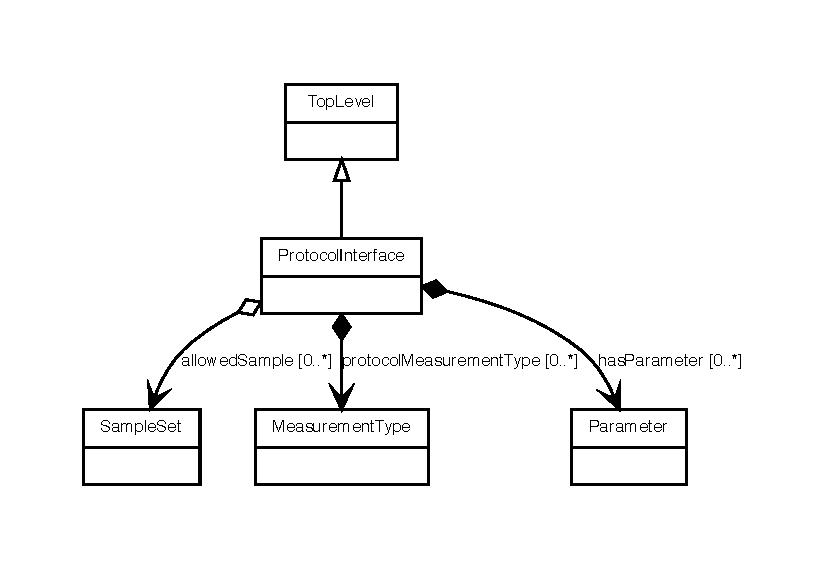
\includegraphics[scale=0.8]{figures/ProtocolInterface}
\caption[]{Diagram of the \opil{ProtocolInterface} class and its associated properties}
\label{uml:ProtocolInterface}
\end{center}
\end{figure}

\begin{itemize}
\item \label{sec:hasSampleSet}
The \opil{hasSampleSet} property MAY contain any number of \opil{URI}s, each of which refers to a \opil{SampleSet} object that describes a range of sample designs allowed for this protocol.
Any sample design whose properties fall into the range defined for any such \opil{SampleSet} SHOULD be accepted for execution of the protocol.
For example, a sample set might indicate that a protocol is intended for use with any strain of {\it E. coli} in any growth media with a concentration of one small-molecule inducer at a concentration between 0 and 1 $\mu$M.

\item \label{sec:hasParameter}
The \opil{hasParameter} property MAY contain any number of \opil{URI}s, each of which refers to a \opil{Parameter} object that describes one of the global parameters used to control the behavior of the protocol. 
For example, a \opil{Parameter} might be used for indicating the range of temperatures that can be requested for a culturing stage or the range of speeds for centrifuging.

\item \label{sec:hasMeasurementType}
The \opil{hasMeasurementType} property MAY contain any number of \opil{URI}s, each of which refers to a \opil{MeasurementType} object that describes a type of instrument that can be used to produce data from this protocol.
For example, a \opil{MeasurementType} might indicate that the protocol can read absorbance from a plate reader up to once every 10 minutes.
\end{itemize}

\subsection{ExperimentalRequest}
\label{sec:ExperimentalRequest}

The \opil{ExperimentalRequest} class is used to describe requests to actually run a particular protocol.

\begin{figure}[ht]
\begin{center}
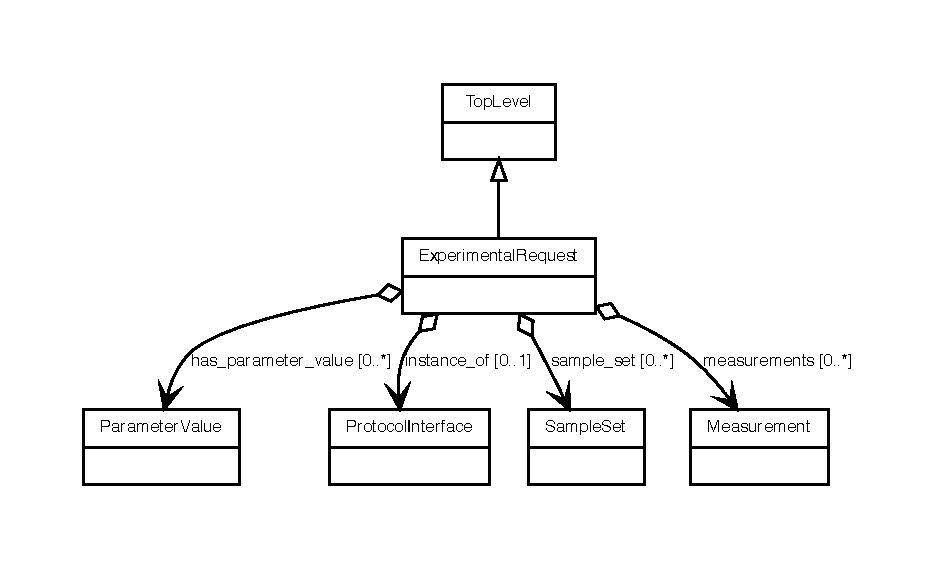
\includegraphics[scale=0.8]{figures/ExperimentalRequest}
\caption[]{Diagram of the \opil{ExperimentalRequest} class and its associated properties}
\label{uml:ExperimentRequest}
\end{center}
\end{figure}

\begin{itemize}
\item \label{sec:ER:instanceOf}
The \opilmult{ER:instanceOf}{instanceOf} property is REQUIRED and MUST contain a single \opil{URI} that refers to the \opil{ProtocolInterface} describing the protocol to be run.

\item \label{sec:hasSampleSet}
The \opil{hasSampleSet} property MAY contain any number of \opil{URI}s, each of which refers to a \opil{SampleSet} object that describes a collection of samples to be run through the experiment.
The total collection of samples requested is the union of all referred \opil{SampleSet} objects.

For example, a sample set might indicate that a protocol is intended for run in triplicate for a positive control strain, negative control strain, and four experimental strains, each at five different levels of inducer and in three different types of media (270 samples), and a second separate sample set might be used to request two replicates each of media-only control for each of the three media (6 samples), for a total of 276 samples.

\item \label{sec:hasMeasurement}
The \opil{hasMeasurement} property MAY contain any number of \opil{URI}s, each of which refers to a \opil{Measurement} object that sets the measurements to be collected during the execution of the protocol.
The total collection of measurements requested is the union of all referred \opil{SampleSet} objects.

For example, a \opil{Measurement} might be used to request plate reader absorbance data be collected at hours 0, 6, and 12, and a second \opil{Measurement} might be used to request that flow cytometry data be collected at hour 12.

\item \label{sec:hasParameterValue}
The \opil{hasParameterValue} property MAY contain any number of \opil{URI}s, each of which refers to a \opil{ParameterValue} object that sets one of the global parameters used to control the behavior of the protocol. 
To prevent conflicts between values, any two \opil{ParameterValue} object thus referred to MUST NOT be a \opil{valueOf} same \opil{Parameter} (e.g., culturing temperature cannot simultaneously be both 30 and  37 degrees Celsius).

For example, a \opil{ParameterValue} might be used to request that culturing temperature be set to 37 degrees Celsius and another used to set centrifuging to 5000 rpm.

\end{itemize}



\subsection{SampleSet}
\label{sec:SampleSet}

The \opil{SampleSet} class is an extension of \sbol{CombinatorialDerivation}, which adds the information of how many replicates should be executed for each specified sample in the combinatorial collection.

\begin{figure}[ht]
\begin{center}
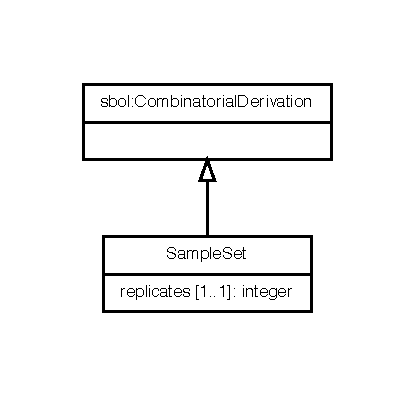
\includegraphics[scale=0.8]{figures/SampleSet}
\caption[]{Diagram of the \opil{SampleSet} class and its associated properties}
\label{uml:SampleSet}
\end{center}
\end{figure}

\begin{itemize}
\item \label{sec:replicates}
The \opil{replicates} property is REQUIRED and MUST contain a single positive \opil{integer} that indicates the number of replicates of each sample that should be run.
\end{itemize}


\subsection{MeasurementType}
\label{sec:MeasurementType}

The \opil{MeasurementType} class is used to indicate when and how often a particular modality of measurement is allowed to be used.
For example, it might be used to say that plate reader data is required to be taken, and that it can be taken up to three times in the range of 12 to 24 hours, no more frequently than once per hour.

\begin{figure}[ht]
\begin{center}
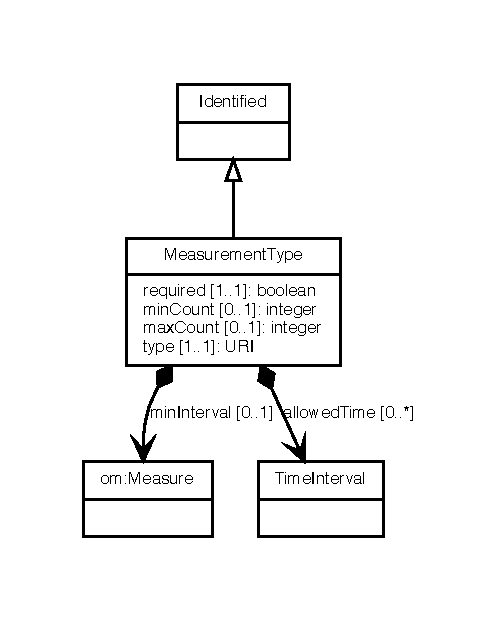
\includegraphics[scale=0.8]{figures/MeasurementType}
\caption[]{Diagram of the \opil{MeasurementType} class and its associated properties}
\label{uml:MeasurementType}
\end{center}
\end{figure}

\todo[inline]{Should we delete the required field, as redundant with minCount?}

\begin{itemize}
\item \label{sec:type}
The \opil{type} property is REQUIRED and MUST contain a \opil{URI} indicating the nature of the measurement being indicated.
When possible, this value SHOULD be drawn from the NCIT ontology's Instrumentation (\url{https://identifiers.org/NCIT:C16742}) or Laboratory Procedure (\url{https://identifiers.org/C25294}) branch.
A list of RECOMMENDED terms for common assays is provided in \ref{tbl:measurement_types}.

\item \label{sec:required}
The \opil{required} property is REQUIRED and MUST contain a \opil{boolean} indicating whether this type of measurement must be used during the execution of the protocol. 
For example, a protocol might always produce plate reader measurements (\opil{required} is true), but have proteomics optional (\opil{required} is false).

\item \label{sec:minCount}
The \opil{minCount} property is OPTIONAL and MAY contain a non-negative \opil{integer} indicating that this \\\opil{MeasurementType} MUST be requested at least the indicated number of times.
If \opil{minCount} is not set, it is treated as zero (or one if \opil{required} is true).
\opil{minCount} must be less than or equal to \opil{maxCount}.

\item \label{sec:maxCount}
The \opil{maxCount} property is OPTIONAL and MAY contain a non-negative \opil{integer} indicating that this \\\opil{MeasurementType} MUST NOT be requested more than the indicated number of times.
If \opil{maxCount} is not set, it is treated as infinity.
\opil{maxCount} must be greater than or equal to \opil{minCount}.


\item \label{sec:minInterval}
The \opil{minInterval} property is OPTIONAL and MAY contain a \opil{URI} referring to a \om{Measure} with a time duration unit indicating the minimum time between two subsequent measurements taken with this modality.
For example, setting \opil{minInterval} to a \om{Measure} specifying one hour would indicate that no two times when this \opil{MeasurementType} is requested may be less than one hour apart.
If \opil{minInterval} is not set, it is treated as zero.

\item \label{sec:allowedTime}
The \opil{allowedTime} property MAY contain any number of \opil{URI}s, each referring to a \opil{TimeInterval} that specifies a range of valid times.
The total set of valid times is the union of all such \opil{TimeInterval}s.
For example, one \opil{TimeInterval} could be used to indicate that the plate reader can be used right at the beginning of the protocol (time 0 hours), then again during the interval of 12 to 24 hours after it began.
If \opil{allowedTime} is not set, then all times are allowed.
\end{itemize}

\begin{table}[ht]
  \begin{edtable}{tabular}{ll}
    \toprule
    \textbf{Measurement Type} & \textbf{URI for NCIT Term} \\
    \midrule
    Flow cytometer & \url{https://identifiers.org/NCIT:C78806}\\
    Microplate reader & \url{https://identifiers.org/NCIT:C70661}\\
    RNAseq & \url{https://identifiers.org/NCIT:C124261}\\
    Fluorescence Microscopy & \url{https://identifiers.org/NCIT:C16856}\\
    \bottomrule
  \end{edtable}
  \caption{Partial list of NCIT terms to specify common assays using the \opil{type} property of a \opil{MeasurementType}}.
 \label{tbl:measurement_types}
\end{table}


\subsubsection{TimeInterval}
\label{sec:TimeInterval}

\todo[inline]{Fold in with factor space, if we do that?}

\opil{TimeInterval} is used for specifying valid ranges of time in which a measurement is allowed to be taken.
For example, it might be used to say that a measurement can be taken anywhere in the range of 12 to 24 hours, or might be used to say that measurements cannot be taken before hour 3.

\begin{figure}[ht]
\begin{center}
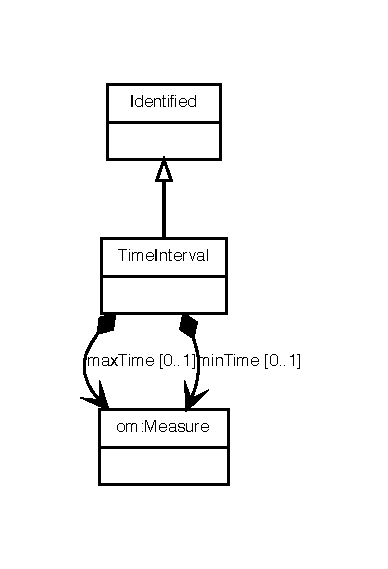
\includegraphics[scale=0.8]{figures/TimeInterval}
\caption[]{Diagram of the \opil{TimeInterval} class and its associated properties}
\label{uml:TimeInterval}
\end{center}
\end{figure}

\begin{itemize}
\item \label{sec:minTime}
The \opil{minTime} property is OPTIONAL and MAY contain a \opil{URI} referring to a \om{Measure} with a time duration unit.
If \opil{minTime} is not set, it is treated as zero.
\opil{minTime} must be less than or equal to \opil{maxTime}.

\item \label{sec:maxTime}
The \opil{maxTime} property is OPTIONAL and MAY contain a \opil{URI} referring to a \om{Measure} with a time duration unit.
If \opil{maxTime} is not set, it is treated as infinity.
\opil{maxTime} must be greater than or equal to \opil{minTime}.
\end{itemize}


\subsection{Measurement}
\label{sec:Measurement}

The \opil{Measurement} class is used to request that a particular measurement be performed at certain times.
For example, it might be used to request that a plate reader be used at hours 0, 6, and 12.

\begin{figure}[ht]
\begin{center}
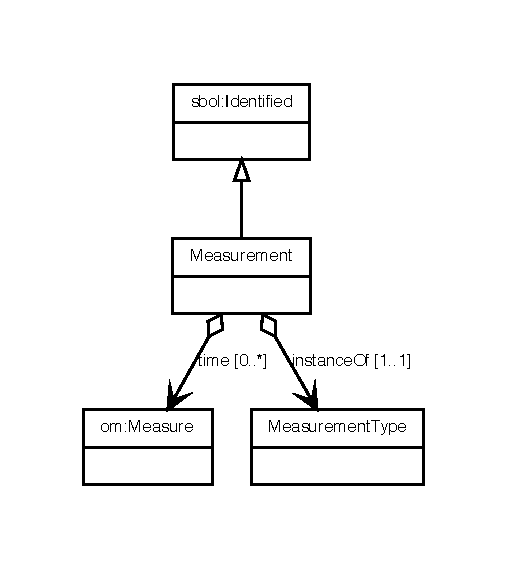
\includegraphics[scale=0.8]{figures/Measurement}
\caption[]{Diagram of the \opil{Measurement} abstract class and its associated properties}
\label{uml:Measurement}
\end{center}
\end{figure}

\begin{itemize}
\item \label{sec:M:instanceOf}
The \opilmult{M:instanceOf}{instanceOf} property is REQUIRED and MUST contain a single \opil{URI} that refers to the \opil{MeasurementType} describing the measurement to be taken.

\item \label{sec:time}
The \opil{time} property MAY contain any number of \opil{URI}s, each referring to a \om{Measure} with a time unit.
\end{itemize}





\subsection{Parameter}
\label{sec:Parameter}

\todo[inline]{Should type be transformed from class type to a field on Parameter, except for the ones that actually have additional fields? This would simplify type-matching validation rules, but add complexity to knowing when an extension is necessary. The EnumeratedParameter allowedValue field could certainly generalize to any. Likewise, the min and max could be generalized for any orderable type (and maybe folded in with factor spaces, if we do that).}
\todo[inline]{I think we need an additional field here to indicate whether a parameter is required or not}

\opil{Parameter} is an abstract class that represents any sort of global setting that may be provided to configure the execution of a protocol.
The subclasses of \opil{Parameter} are used to indicate different types of value to be set, such as Booleans, integers, and measures (i.e., floating point values with units).

This is a catch-all class intended for capturing any information that cannot be systematized in terms of \opil{SampleSet} and \opil{Measurement} information, and thus SHOULD NOT be used to represent anything that can be well-represented using those classes.

For example, a \opil{Parameter} can be used to determine whether an optional post-culturing dilution step should be executed.
A \opil{Parameter} SHOULD NOT be used to determine which culture media should be used in a sample (since that can be represented well via \opil{SampleSet}) or to indicate whether samples should be evaluated with an optional proteomics step (since that can be represented well via \opil{Measurement}).



\begin{figure}[ht]
\begin{center}
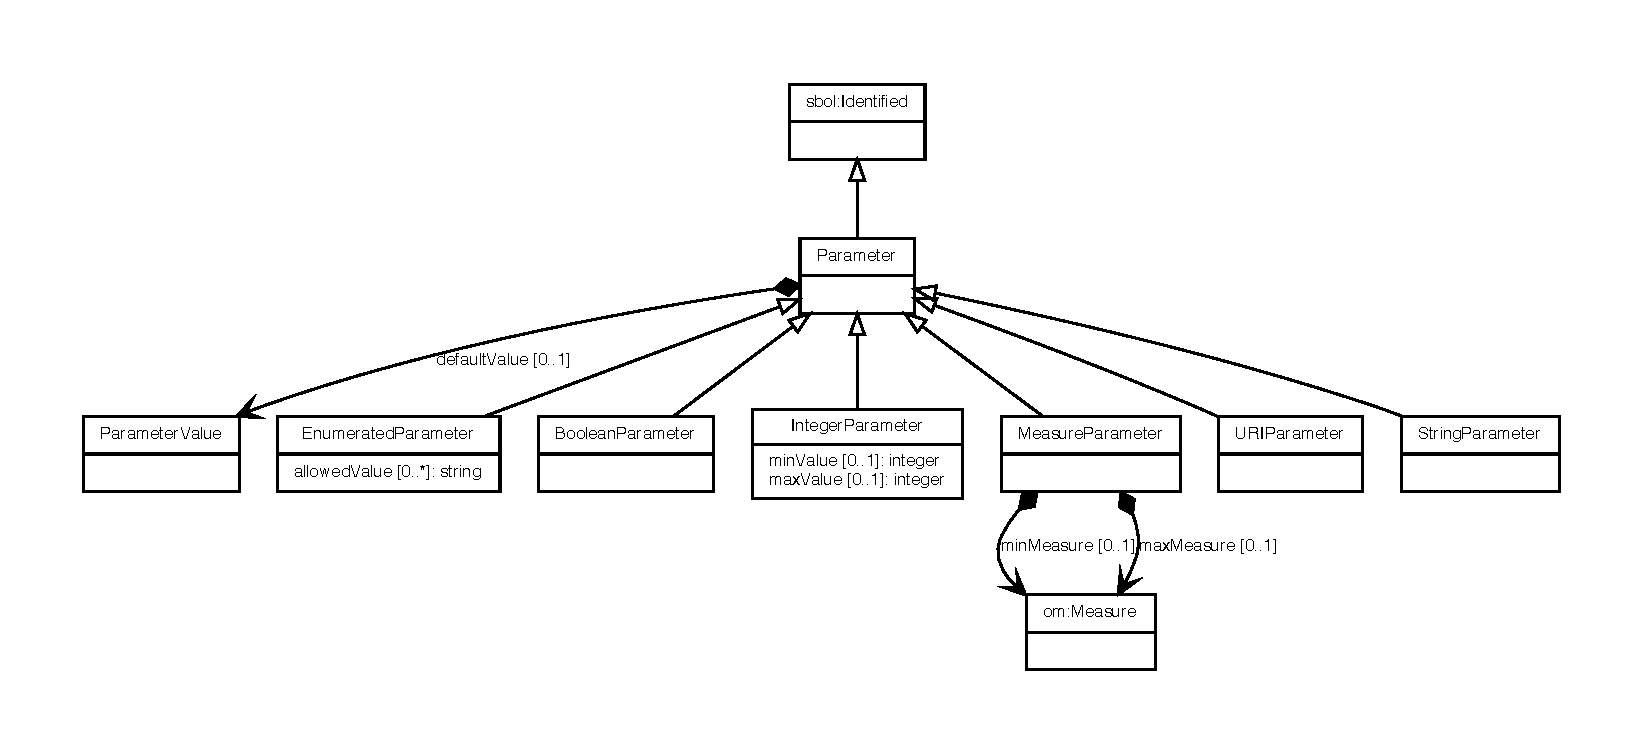
\includegraphics[scale=0.6]{figures/Parameter_definition_and_abstraction}
\caption[]{Diagram of the \opil{Parameter} abstract class and its associated properties and subclasses}
\label{uml:Parameter}
\end{center}
\end{figure}

\begin{itemize}
\item \label{sec:defaultValue}
The \opil{defaultValue} property is OPTIONAL and MAY contain a single \opil{URI} that refers to a \opil{ParameterValue} that provides a default value for the parameter in the case that it is not set.
\end{itemize}


\subsubsection{BooleanParameter}
\label{sec:BooleanParameter}

{\em \opil{BooleanParameter} has no additional properties.}

\subsubsection{EnumeratedParameter}
\label{sec:EnumeratedParameter}

\begin{itemize}
\item \label{sec:allowedValue}
The \opil{allowedValue} property MAY contain any number of \opil{string} values, indicating the legal values for this \opil{EnumeratedParameter}. 
For example, 
\end{itemize}

\subsubsection{IntegerParameter}
\label{sec:IntegerParameter}

\begin{itemize}
\item \label{sec:minValue}
The \opil{minValue} property is OPTIONAL and MAY contain an \opil{integer}.
If \opil{minValue} is not set, it is treated as negative infinity.
\opil{minValue} must be less than or equal to \opil{maxValue}.

\item \label{sec:maxValue}
The \opil{maxValue} property is OPTIONAL and MAY contain an \opil{integer}.
If \opil{maxValue} is not set, it is treated as infinity.
\opil{maxValue} must be greater than or equal to \opil{minValue}.
\end{itemize}

\subsubsection{MeasureParameter}
\label{sec:MeasureParameter}

\begin{itemize}
\item \label{sec:minMeasure}
The \opil{minMeasure} property is OPTIONAL and MAY contain a \opil{URI} referring to a \om{Measure}.
If \opil{minMeasure} is not set, it is treated as negative infinity.
\opil{minMeasure} must be less than or equal to \opil{maxMeasure}.

\item \label{sec:maxMeasure}
The \opil{maxMeasure} property is OPTIONAL and MAY contain a \opil{URI} referring to a \om{Measure}.
If \opil{maxMeasure} is not set, it is treated as infinity.
\opil{maxMeasure} must be greater than or equal to \opil{minMeasure}.
\end{itemize}

\subsubsection{StringParameter}
\label{sec:StringParameter}

{\em \opil{BooleanParameter} has no additional properties.}

\subsubsection{URIParameter}
\label{sec:URIParameter}

{\em \opil{BooleanParameter} has no additional properties.}


\subsection{ParameterValue}
\label{sec:ParameterValue}

\opil{ParameterValue} is an abstract class is used to set a parameter for a protocol to a particular value. 
The subclasses of \opil{ParameterValue} are used for different types of value to be set, such as Booleans, integers, and measures (i.e., floating point values with units).
For example, a \opil{MeasureValue} might be used to request that a centrifuging step be run at 5000 rpm.

\begin{figure}[ht]
\begin{center}
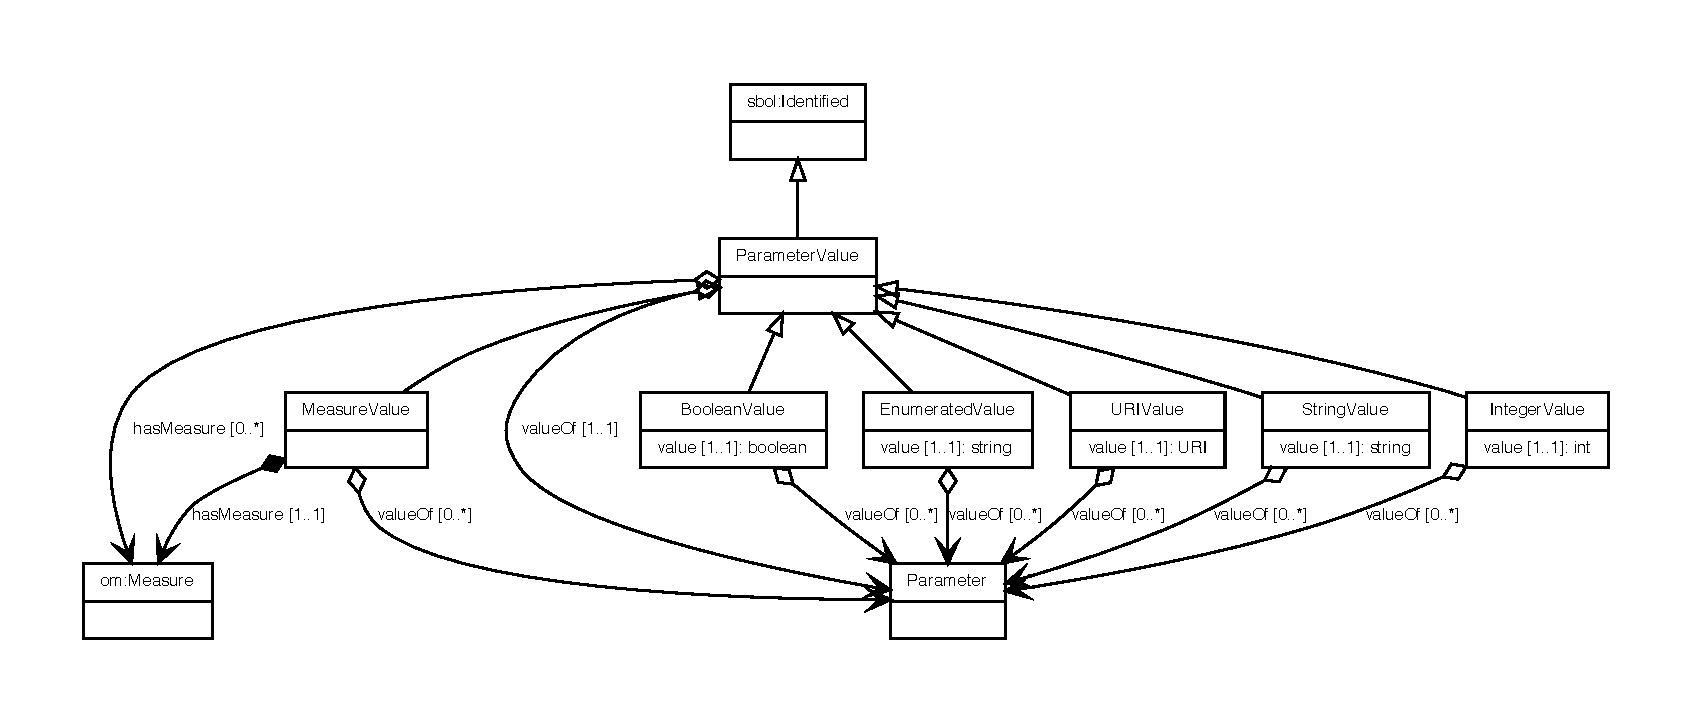
\includegraphics[scale=0.6]{figures/ParameterValue_definition_and_abstraction}
\caption[]{Diagram of the \opil{ParameterValue} abstract class and its associated properties and subclasses}
\label{uml:ParameterValue}
\end{center}
\end{figure}

\begin{itemize}
\item \label{sec:valueOf}
The \opil{valueOf} property is REQUIRED and MUST contain a single \opil{URI} that refers to the \opil{Parameter} describing the parameter being set.
The \opil{Parameter} MUST be of a corresponding class, e.g., a \opil{BooleanValue} must match a \opil{BooleanParameter}.
\end{itemize}


\subsubsection{BooleanValue}
\label{sec:BooleanValue}

\begin{itemize}
\item \label{sec:BP:value}
The \opilmult{BP:value}{value} property is REQUIRED and MUST contain a single \opil{boolean}.
\end{itemize}

\subsubsection{EnumeratedValue}
\label{sec:EnumeratedValue}

\begin{itemize}
\item \label{sec:EV:value}
The \opilmult{EV:value}{value} property is REQUIRED and MUST contain a single \opil{string} whose value is equal to one of the \opil{allowedValue} properties of the \opil{Parameter} referred to by the \opil{valueOf} property.
\end{itemize}


\subsubsection{IntegerValue}
\label{sec:IntegerValue}

\begin{itemize}
\item \label{sec:IV:value}
The \opilmult{IV:value}{value} property is REQUIRED and MUST contain a single \opil{integer}.
The value must be greater than or equal to that of the \opil{minValue} property (if set) of the \opil{Parameter} referred to by the \opil{valueOf} property, and less than or equal to the \opil{maxValue} property (if set).
\end{itemize}

\subsubsection{MeasureValue}
\label{sec:MeasureValue}

\begin{itemize}
\item \label{sec:hasValue}
The \opil{hasValue} property is REQUIRED and MUST contain a single \opil{URI} referring to a \om{Measure} object containing the value for the parameter.
The value of the linked \om{Measure} must be greater than or equal to that of the \opil{minMeasure} property (if set) of the \opil{Parameter} referred to by the \opil{valueOf} property, and less than or equal to the \opil{maxMeasure} property (if set).
\end{itemize}


\subsubsection{StringValue}
\label{sec:StringValue}

\begin{itemize}
\item \label{sec:SV:value}
The \opilmult{SV:value}{value} property is REQUIRED and MUST contain a single \opil{string}.
\end{itemize}


\subsubsection{URIValue}
\label{sec:URIValue}

\begin{itemize}
\item \label{sec:UV:value}
The \opilmult{UV:value}{value} property is REQUIRED and MUST contain a single \opil{URI}.
\end{itemize}












\section{Serialization}
\label{sec:serialization}

In order for OPIL objects to be readily stored and exchanged, it is important that they are able to be {\em serialized}, i.e., converted to a sequence of bytes that can be stored in a file or exchanged over a network.  
%
To this end, OPIL builds upon the Resource Description Framework (RDF).  RDF is an abstract language for describing conceptual graph-oriented data models, and therefore does not mandate any specific serialization format.  Instead, a number of different serialization formats are provided as separate specifications, such as RDF/XML, N-Triples, JSON-LD, and Turtle.  These serialization formats are widely supported by RDF libraries such as rdflib for Python and Apache Jena for Java.

All OPIL libraries SHOULD support at least RDF/XML, N-Triples, JSON-LD, and Turtle.
Other OPIL tools SHOULD support at least one of these four formats.


\newpage
\bibliography{opil}

\appendix

%\input{examples}

\end{document}
